\section{Analysis}\label{sec:caida_results}

The following sections describe analysis of the \caida and \ripe Atlas data in a natural progression from analysis of data quality, to basic connectivity analysis, and finally to geographic plotting and \gis tooling.

\subsection{Data Quality}\label{sec:caida_data_quality}

To determine the quality of the data, we made a series of \kde charts with the Python library \textit{seaborn} \cite{seaborn}. Since histograms are vulnerable to binning effects and cumulative distribution charts tend to be less intuitive to read, distributions in this report are presented as \acrfull{kde} charts. Briefly, these work by drawing a Gaussian distribution around each point of data, summing all distributions together, and normalizing so the area under the curve is equal to 1. The $y$ axis, then, does not represent a real value, instead only a probability density. \KDE charts contrast \cdf charts which can be used to more easily extract median, percentiles, etc.; however, the point of the charts here is more to show clustering than anything, which \kde charts excel at intuitively presenting.

% \begin{wrapfigure}[16]{L}{0.65\textwidth}
\begin{figure}[t]
    \centering
    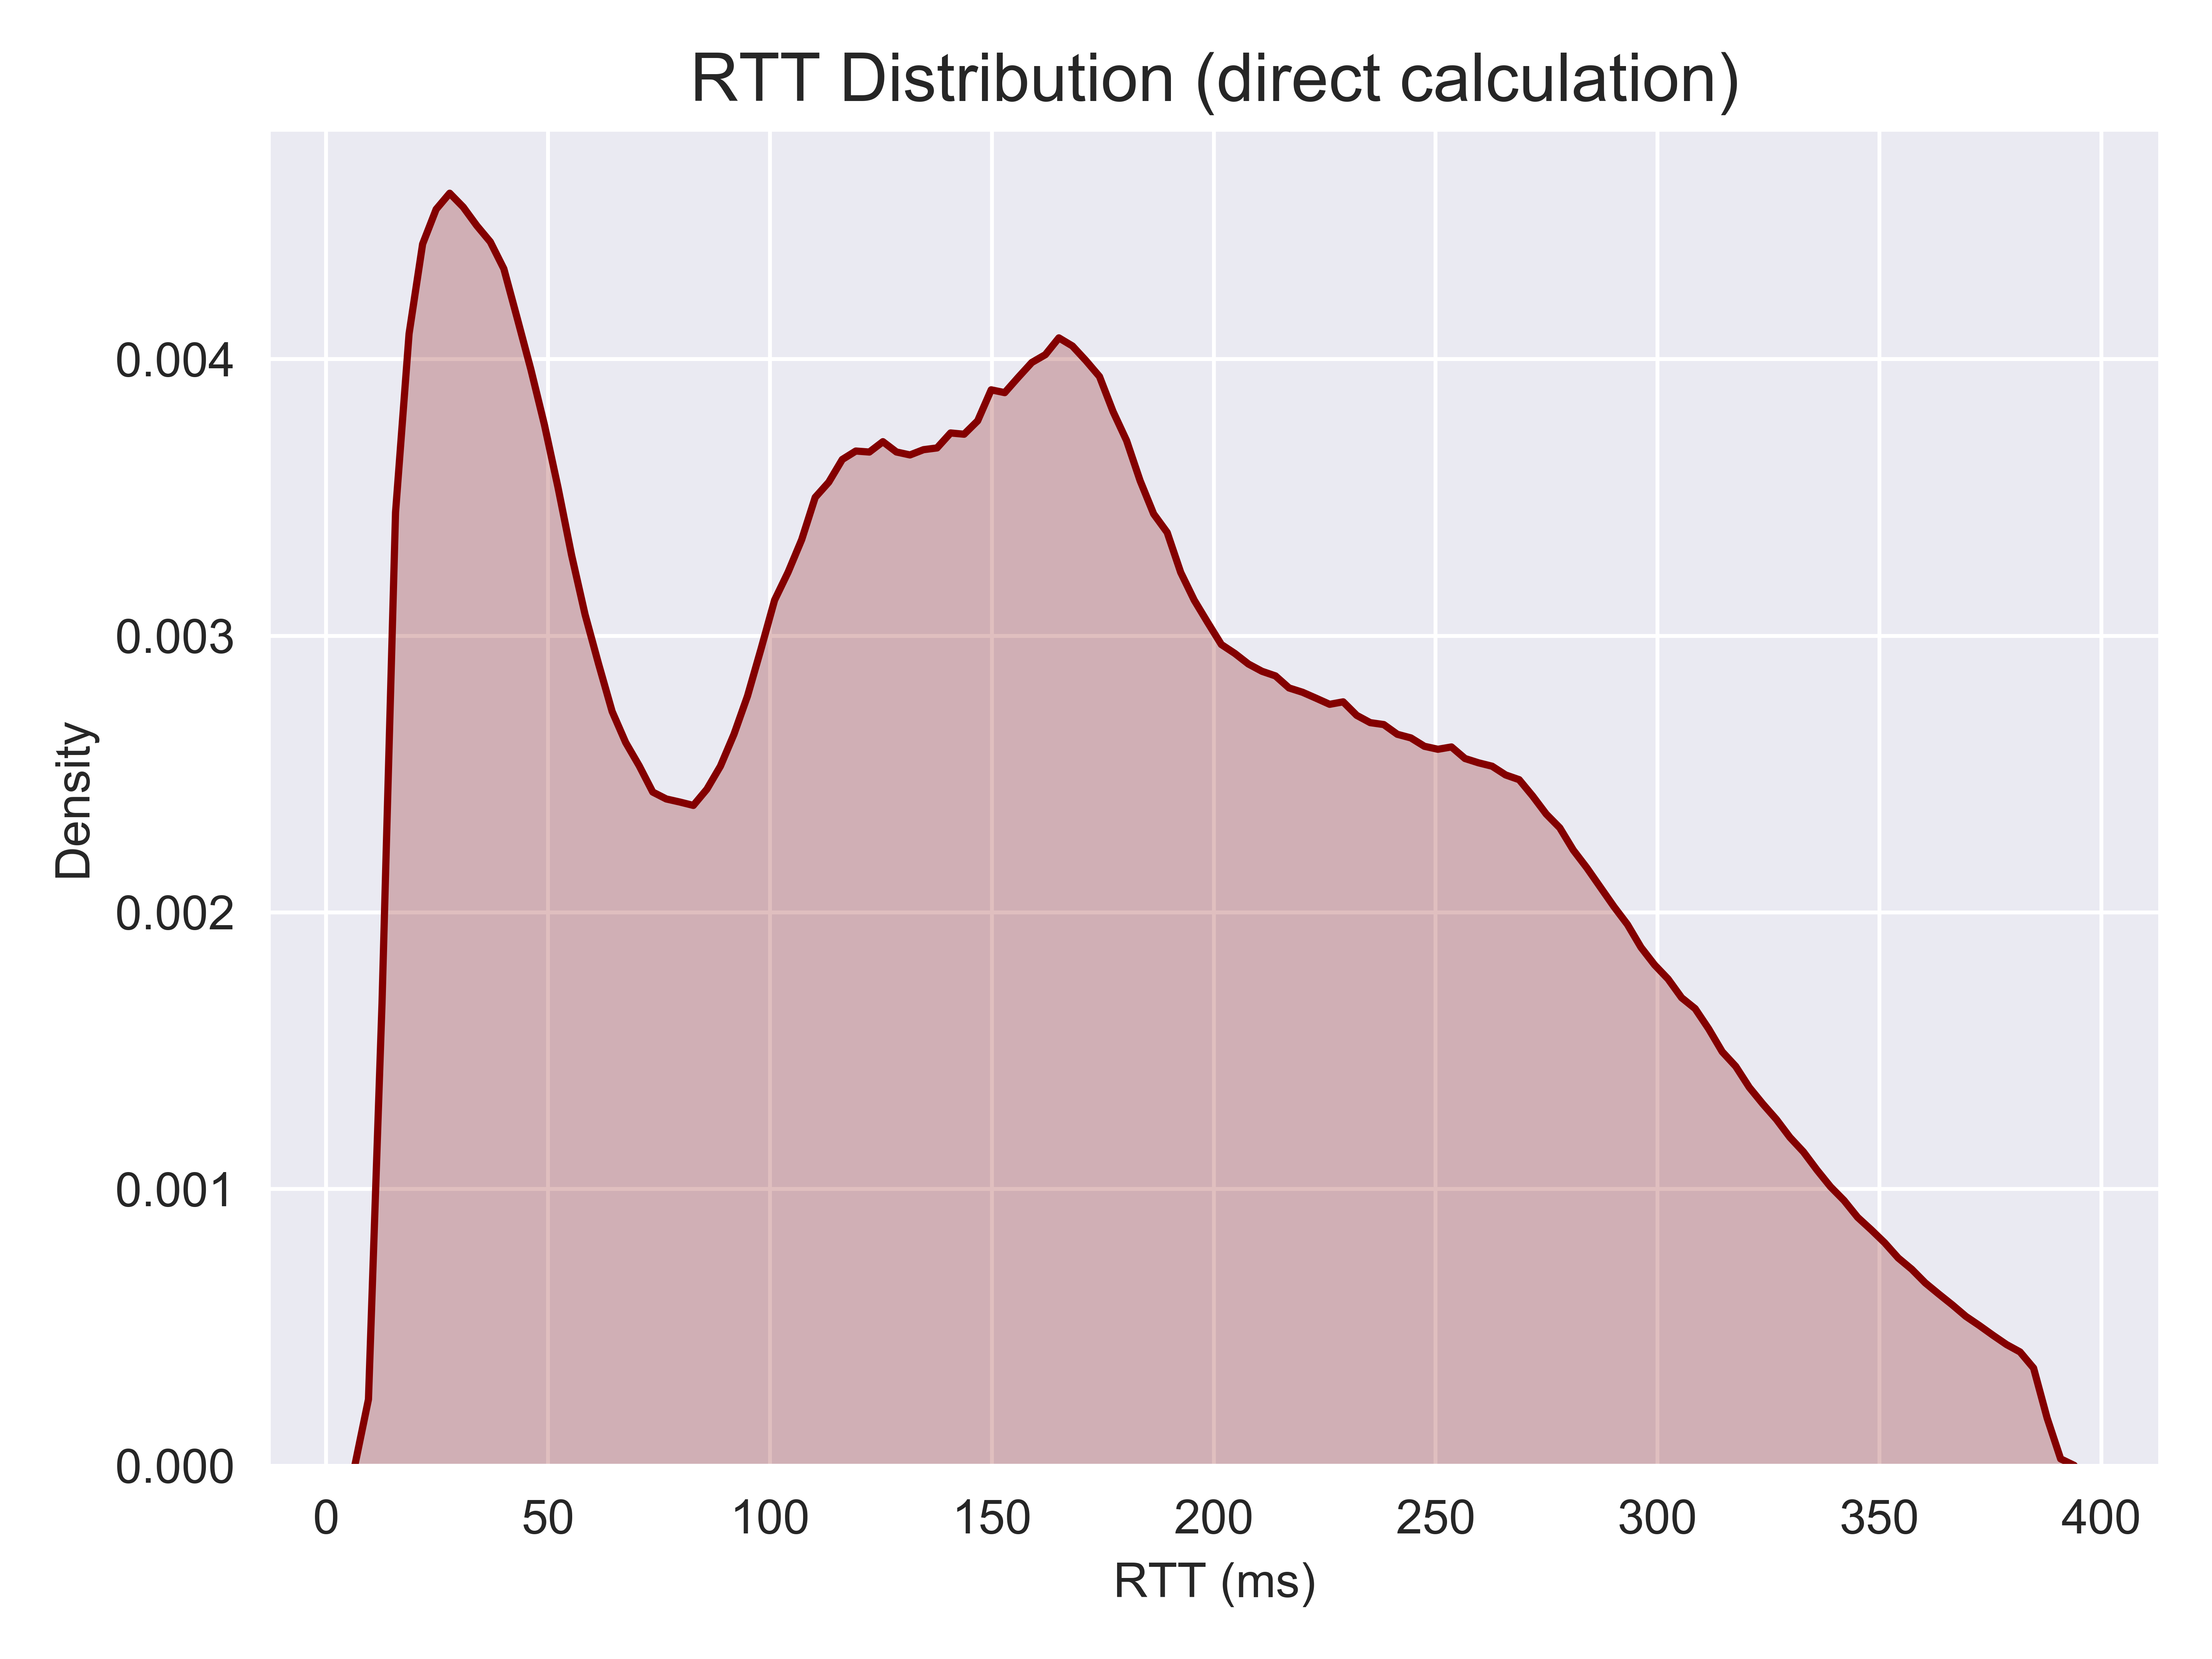
\includegraphics[width=0.65\textwidth]{caida/rtt_distribution.png}
    \caption{RTT distribution, direct ping calculation}
    \label{fig:caida_rtt_distribution}
\end{figure}
% \end{wrapfigure}

The most immediately useful distribution is that of the \rtt between \ip pairs, shown for direct-calculated \rtts in \cref{fig:caida_rtt_distribution}. The distribution appears weakly bimodal, which we hypothesize is due to the global nature of \ripe Atlas and \caida's individual measurement networks. The leftmost peak corresponds to measurements to a device that shares a land mass with the device performing the traceroute, while the rightmost peak corresponds to a combination of devices on a different land mass and devices with lower-performing connections. \Cref{fig:caida_distance_distribution} appears to confirm this hypothesis, since it too is similarly bimodal.

% \begin{wrapfigure}[15]{L}{0.65\textwidth}
\begin{figure}[htb]
    \centering
    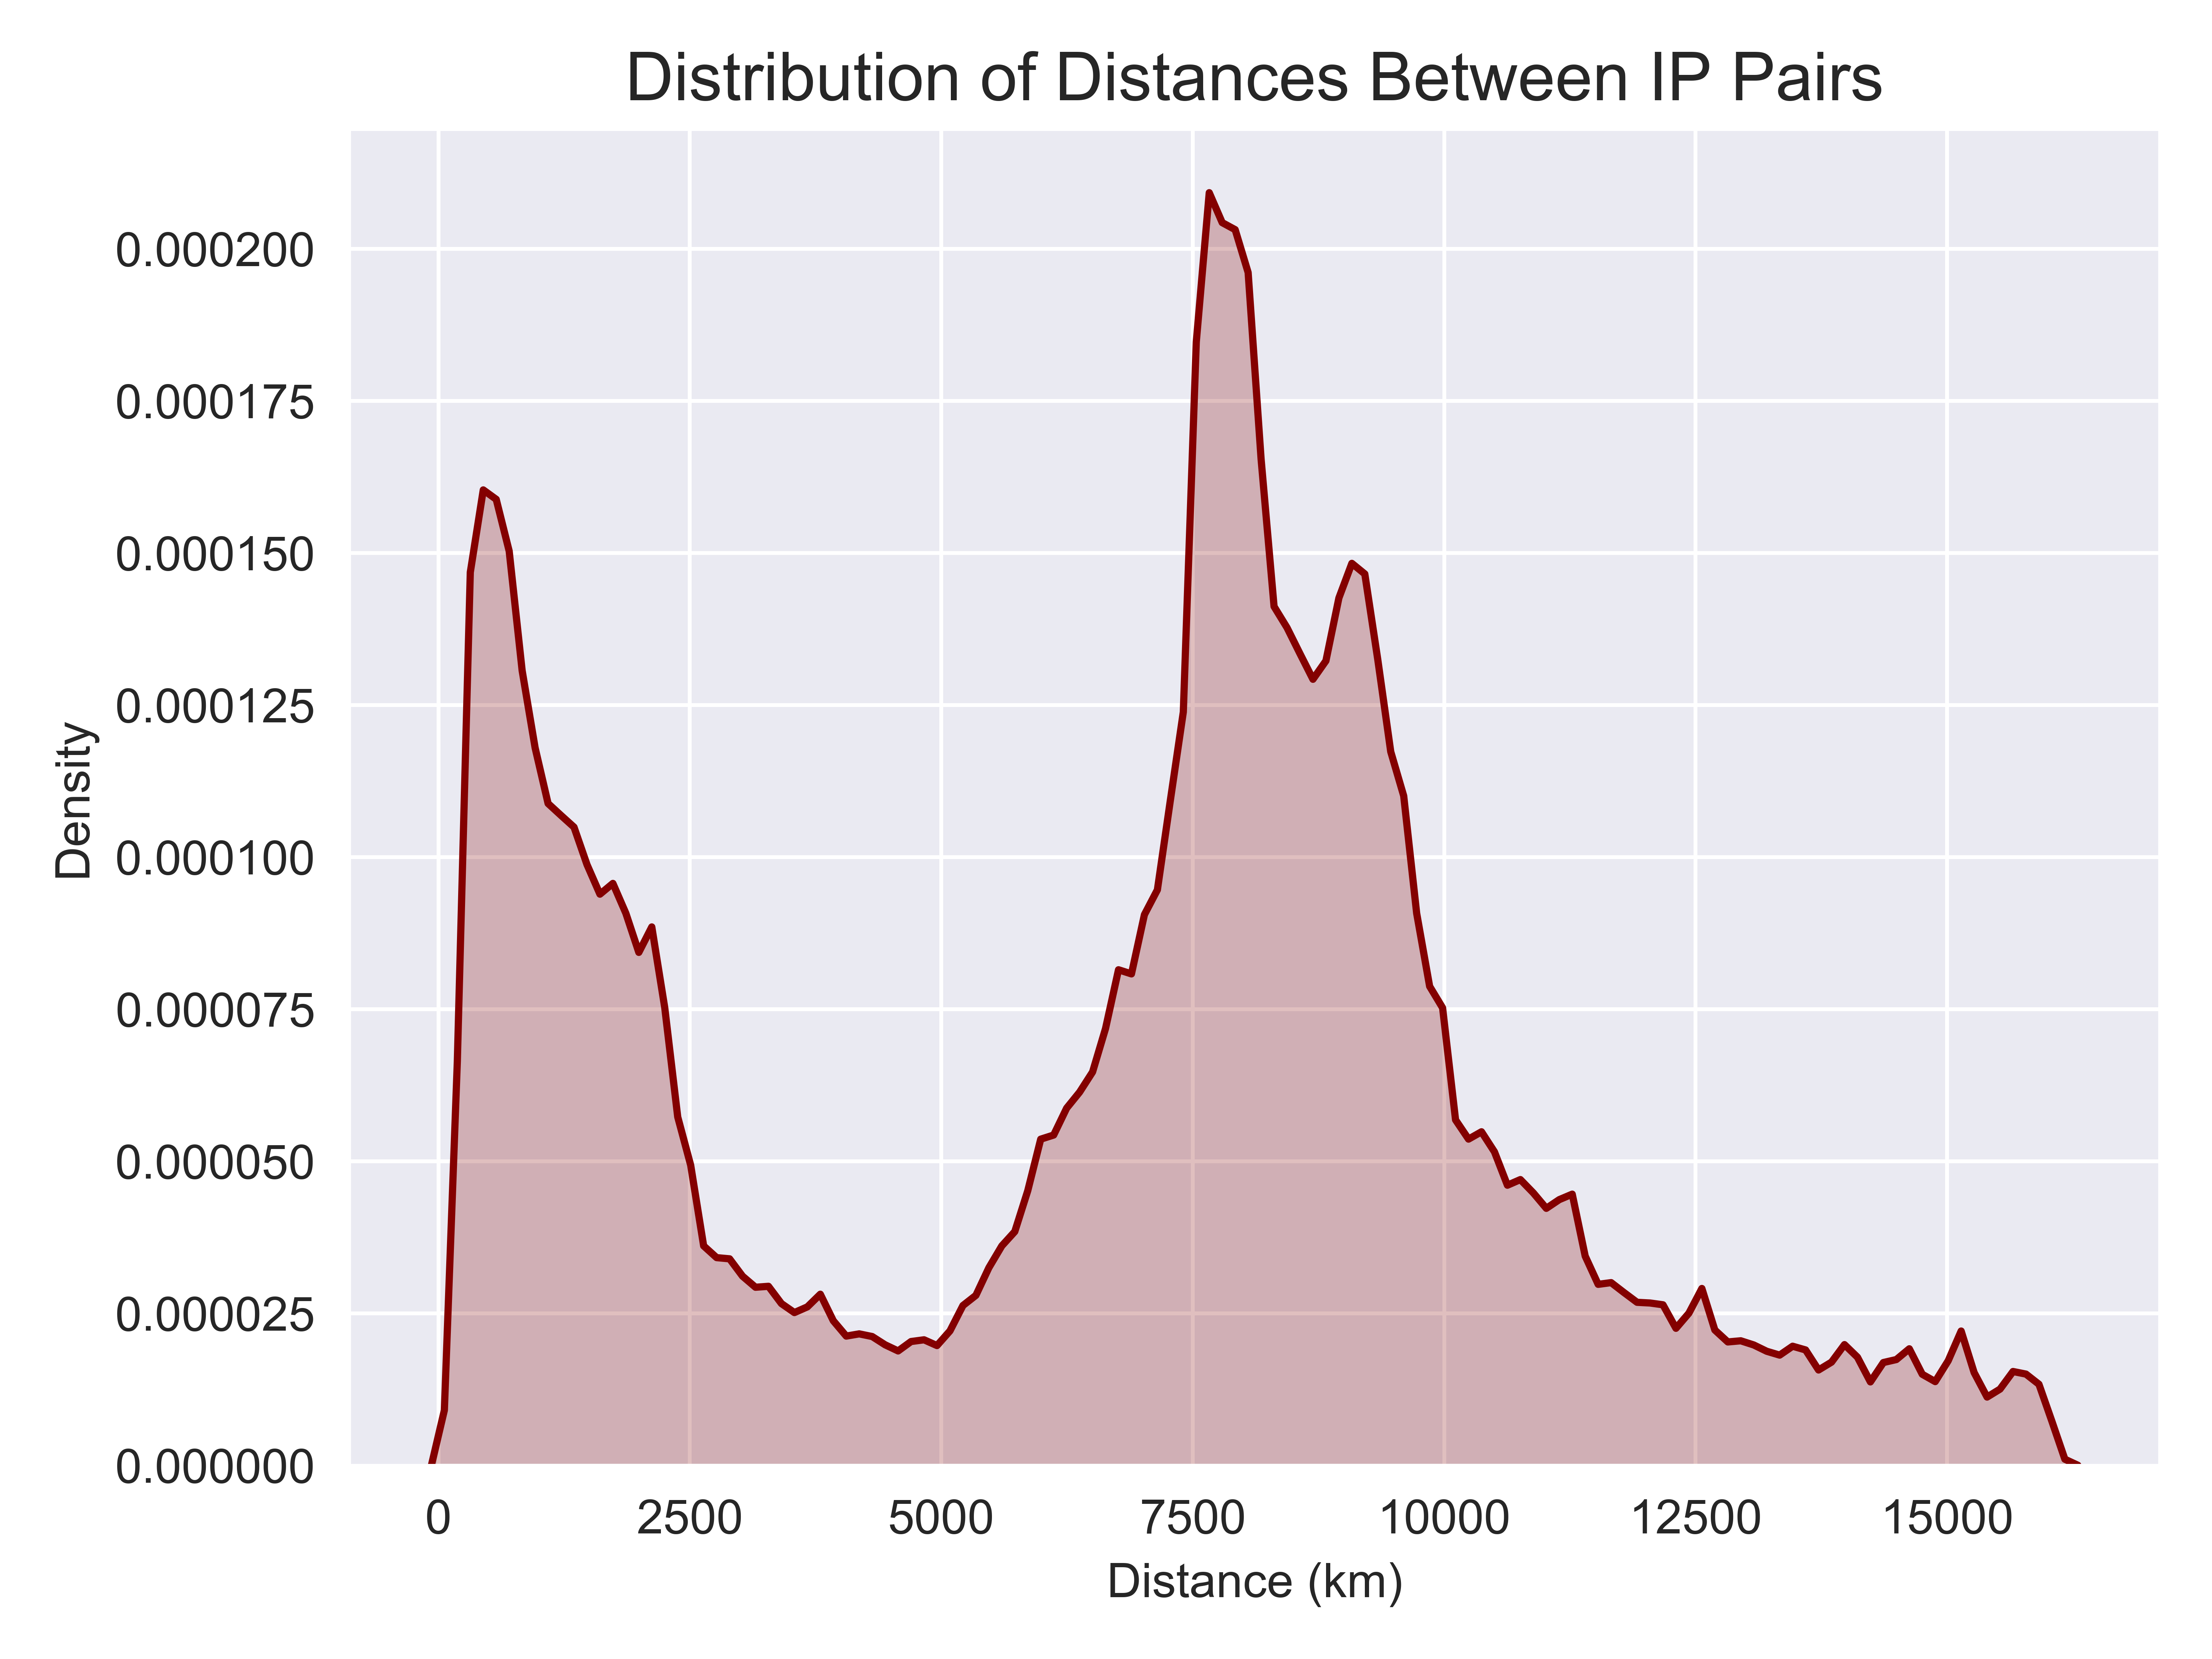
\includegraphics[width=0.65\textwidth]{caida/distance_distribution.png}
    \caption{Address pair distance distribution}
    \label{fig:caida_distance_distribution}
\end{figure}
% \end{wrapfigure}

 \Cref{fig:caida_rtt_distribution_indirect} shows the distribution of \rtts calculated using the indirect ping calculation method, of which a calculated \textapprox29\% are below zero -- an impossible value. Since a significant fraction of the data points are completely impossible it was decided that this data was too unreliable for further analysis. The remainder of the data analyses in this section are based on the direct ping calculation method only.

% \begin{wrapfigure}[18]{l}{0.65\textwidth}
\begin{figure}[htb]
    \centering
    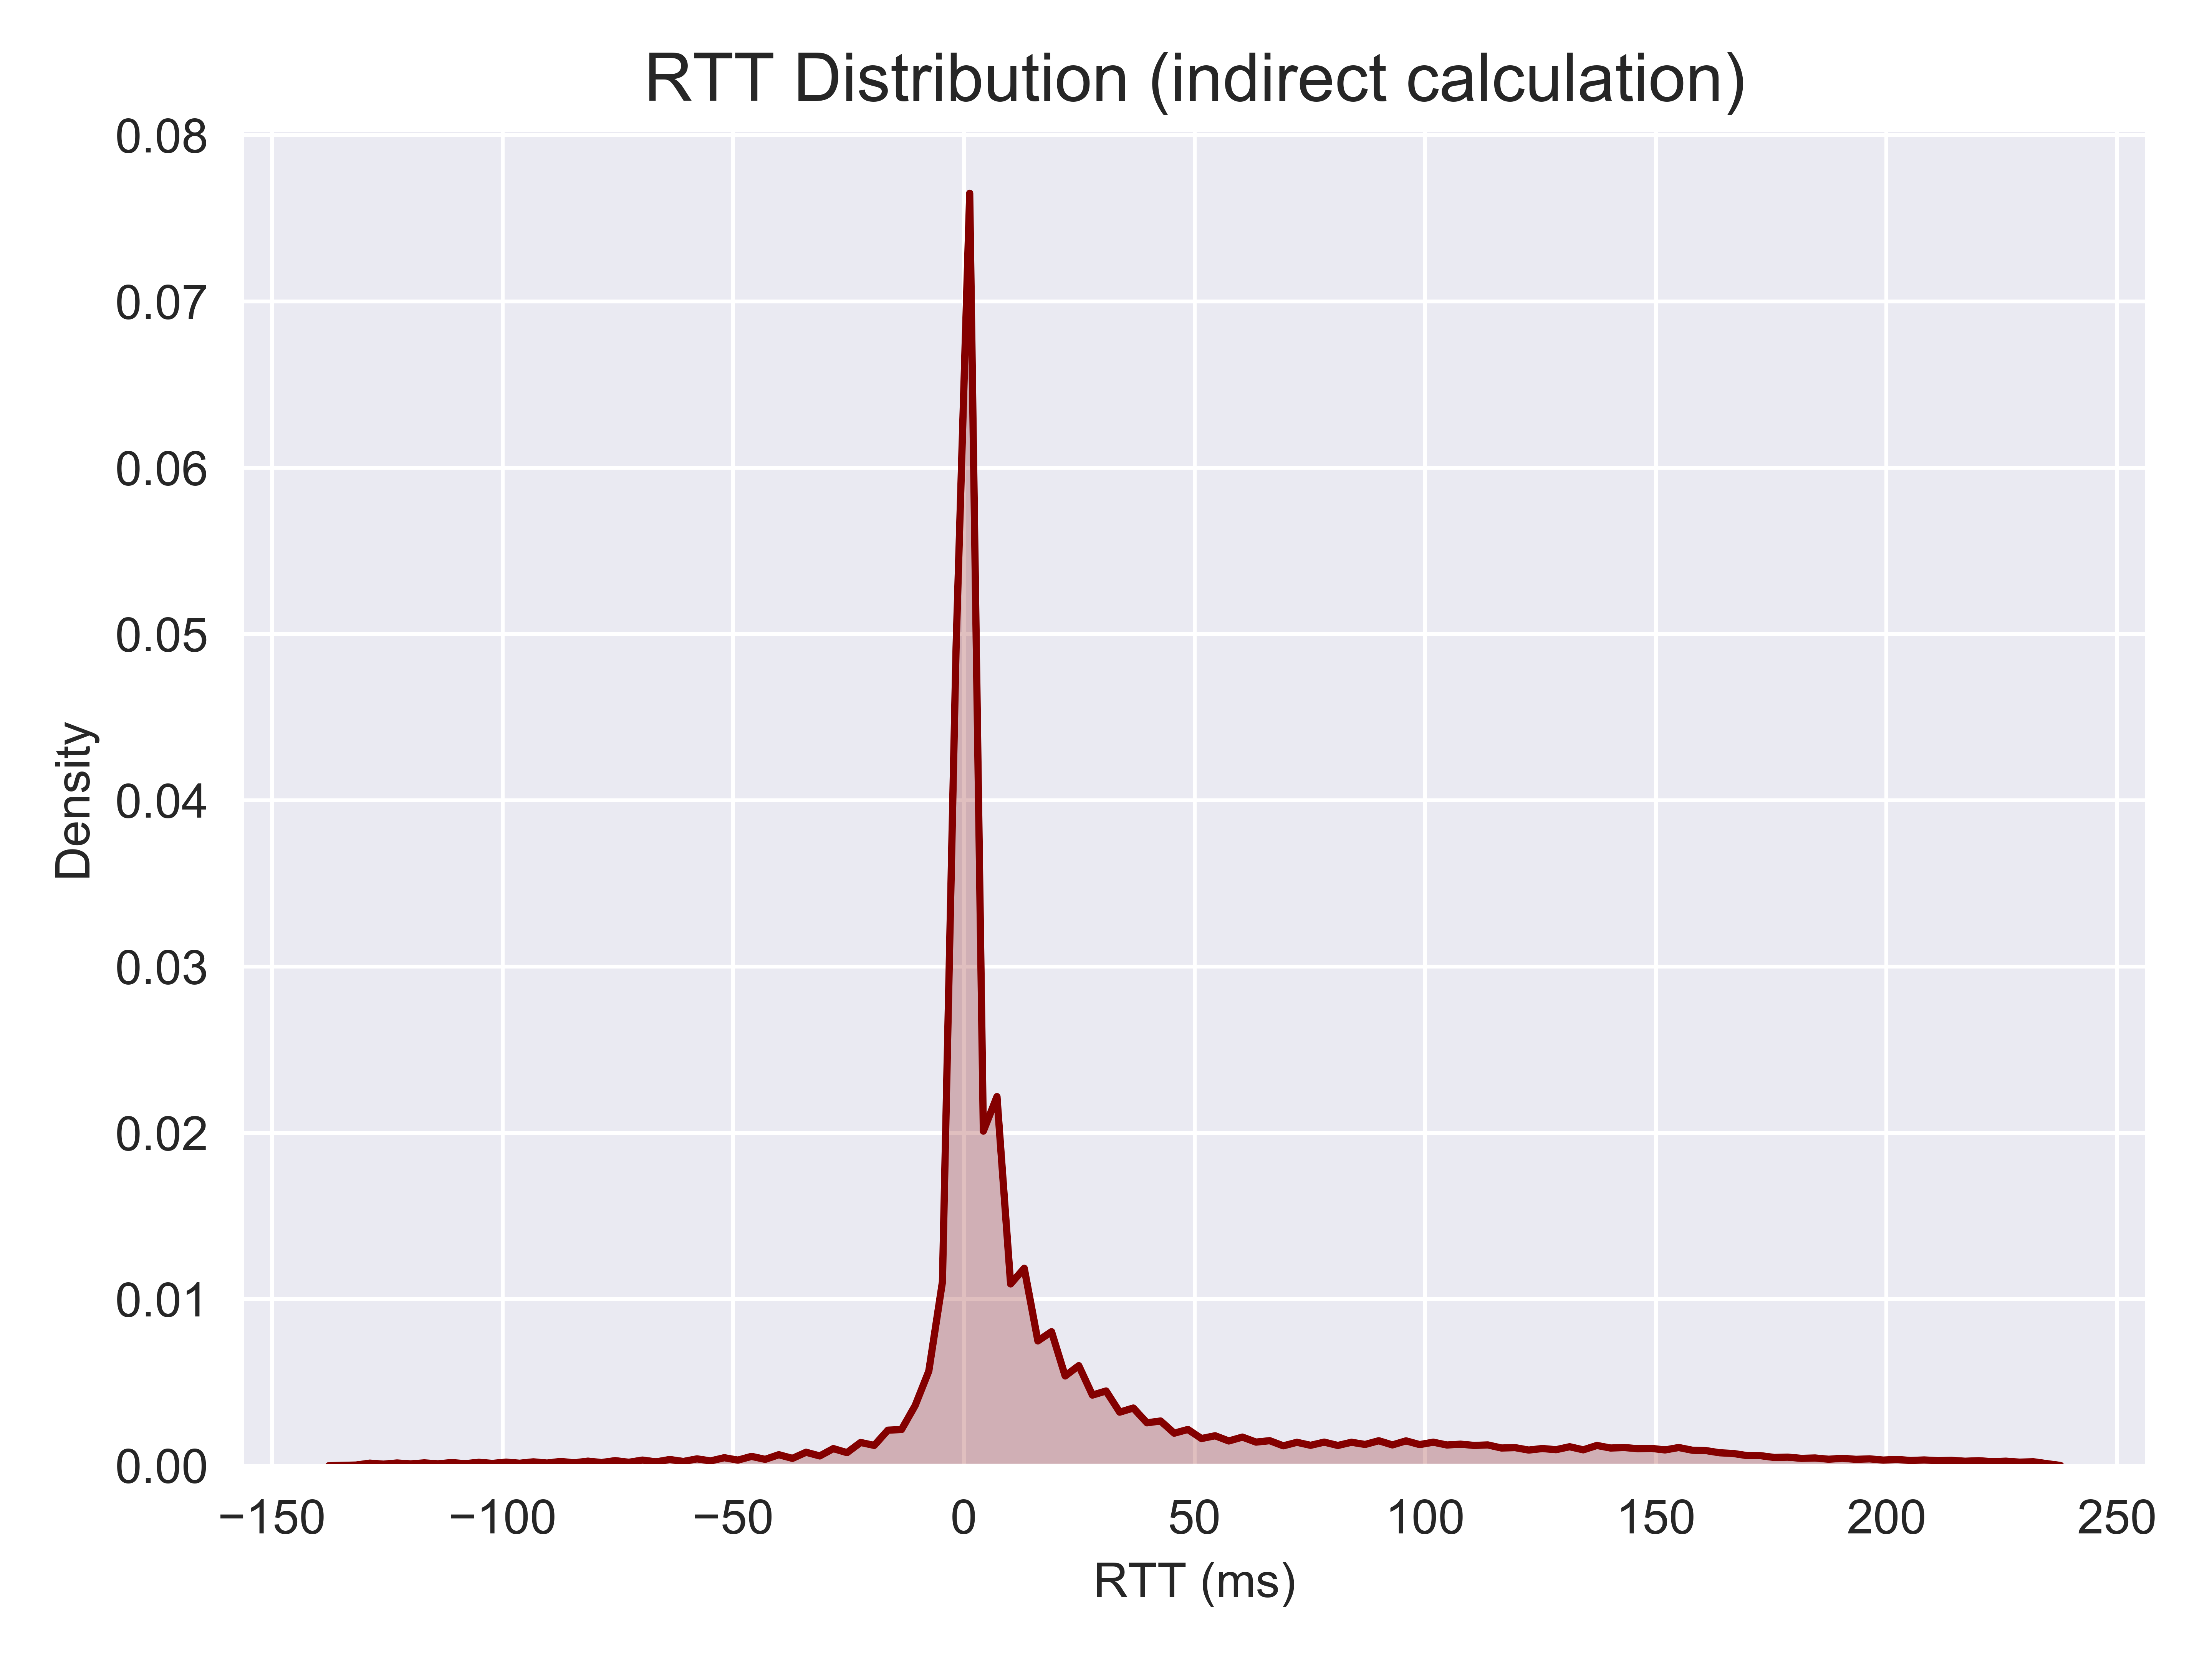
\includegraphics[width=0.65\textwidth]{caida/rtt_distribution_indirect.png}
    \caption{Distribution of RTT between IP pairs, indirect ping calculation}
    \label{fig:caida_rtt_distribution_indirect}
\end{figure}
% \end{wrapfigure}

To further assess data quality we turned to measures of the data spread for each data point. \Cref{fig:caida_measurements_distribution} shows the distribution of measurement counts between each \ip address pair, showing that although most pairs had on the order of 1-20 measurements, a sizeable fraction had more than that, and there were even some in the 500+ measurements range. This effect is likely a result of the way \ripe Atlas and \caida nodes are networked. A node's local gateway would always show up on a traceroute (unless configured to not respond to pings), as would common paths through a node's \isp, so these \ip addresses are measured extremely frequently.

% \begin{wrapfigure}{R}{0.4\textwidth}
\begin{figure}[htb]
    \centering
    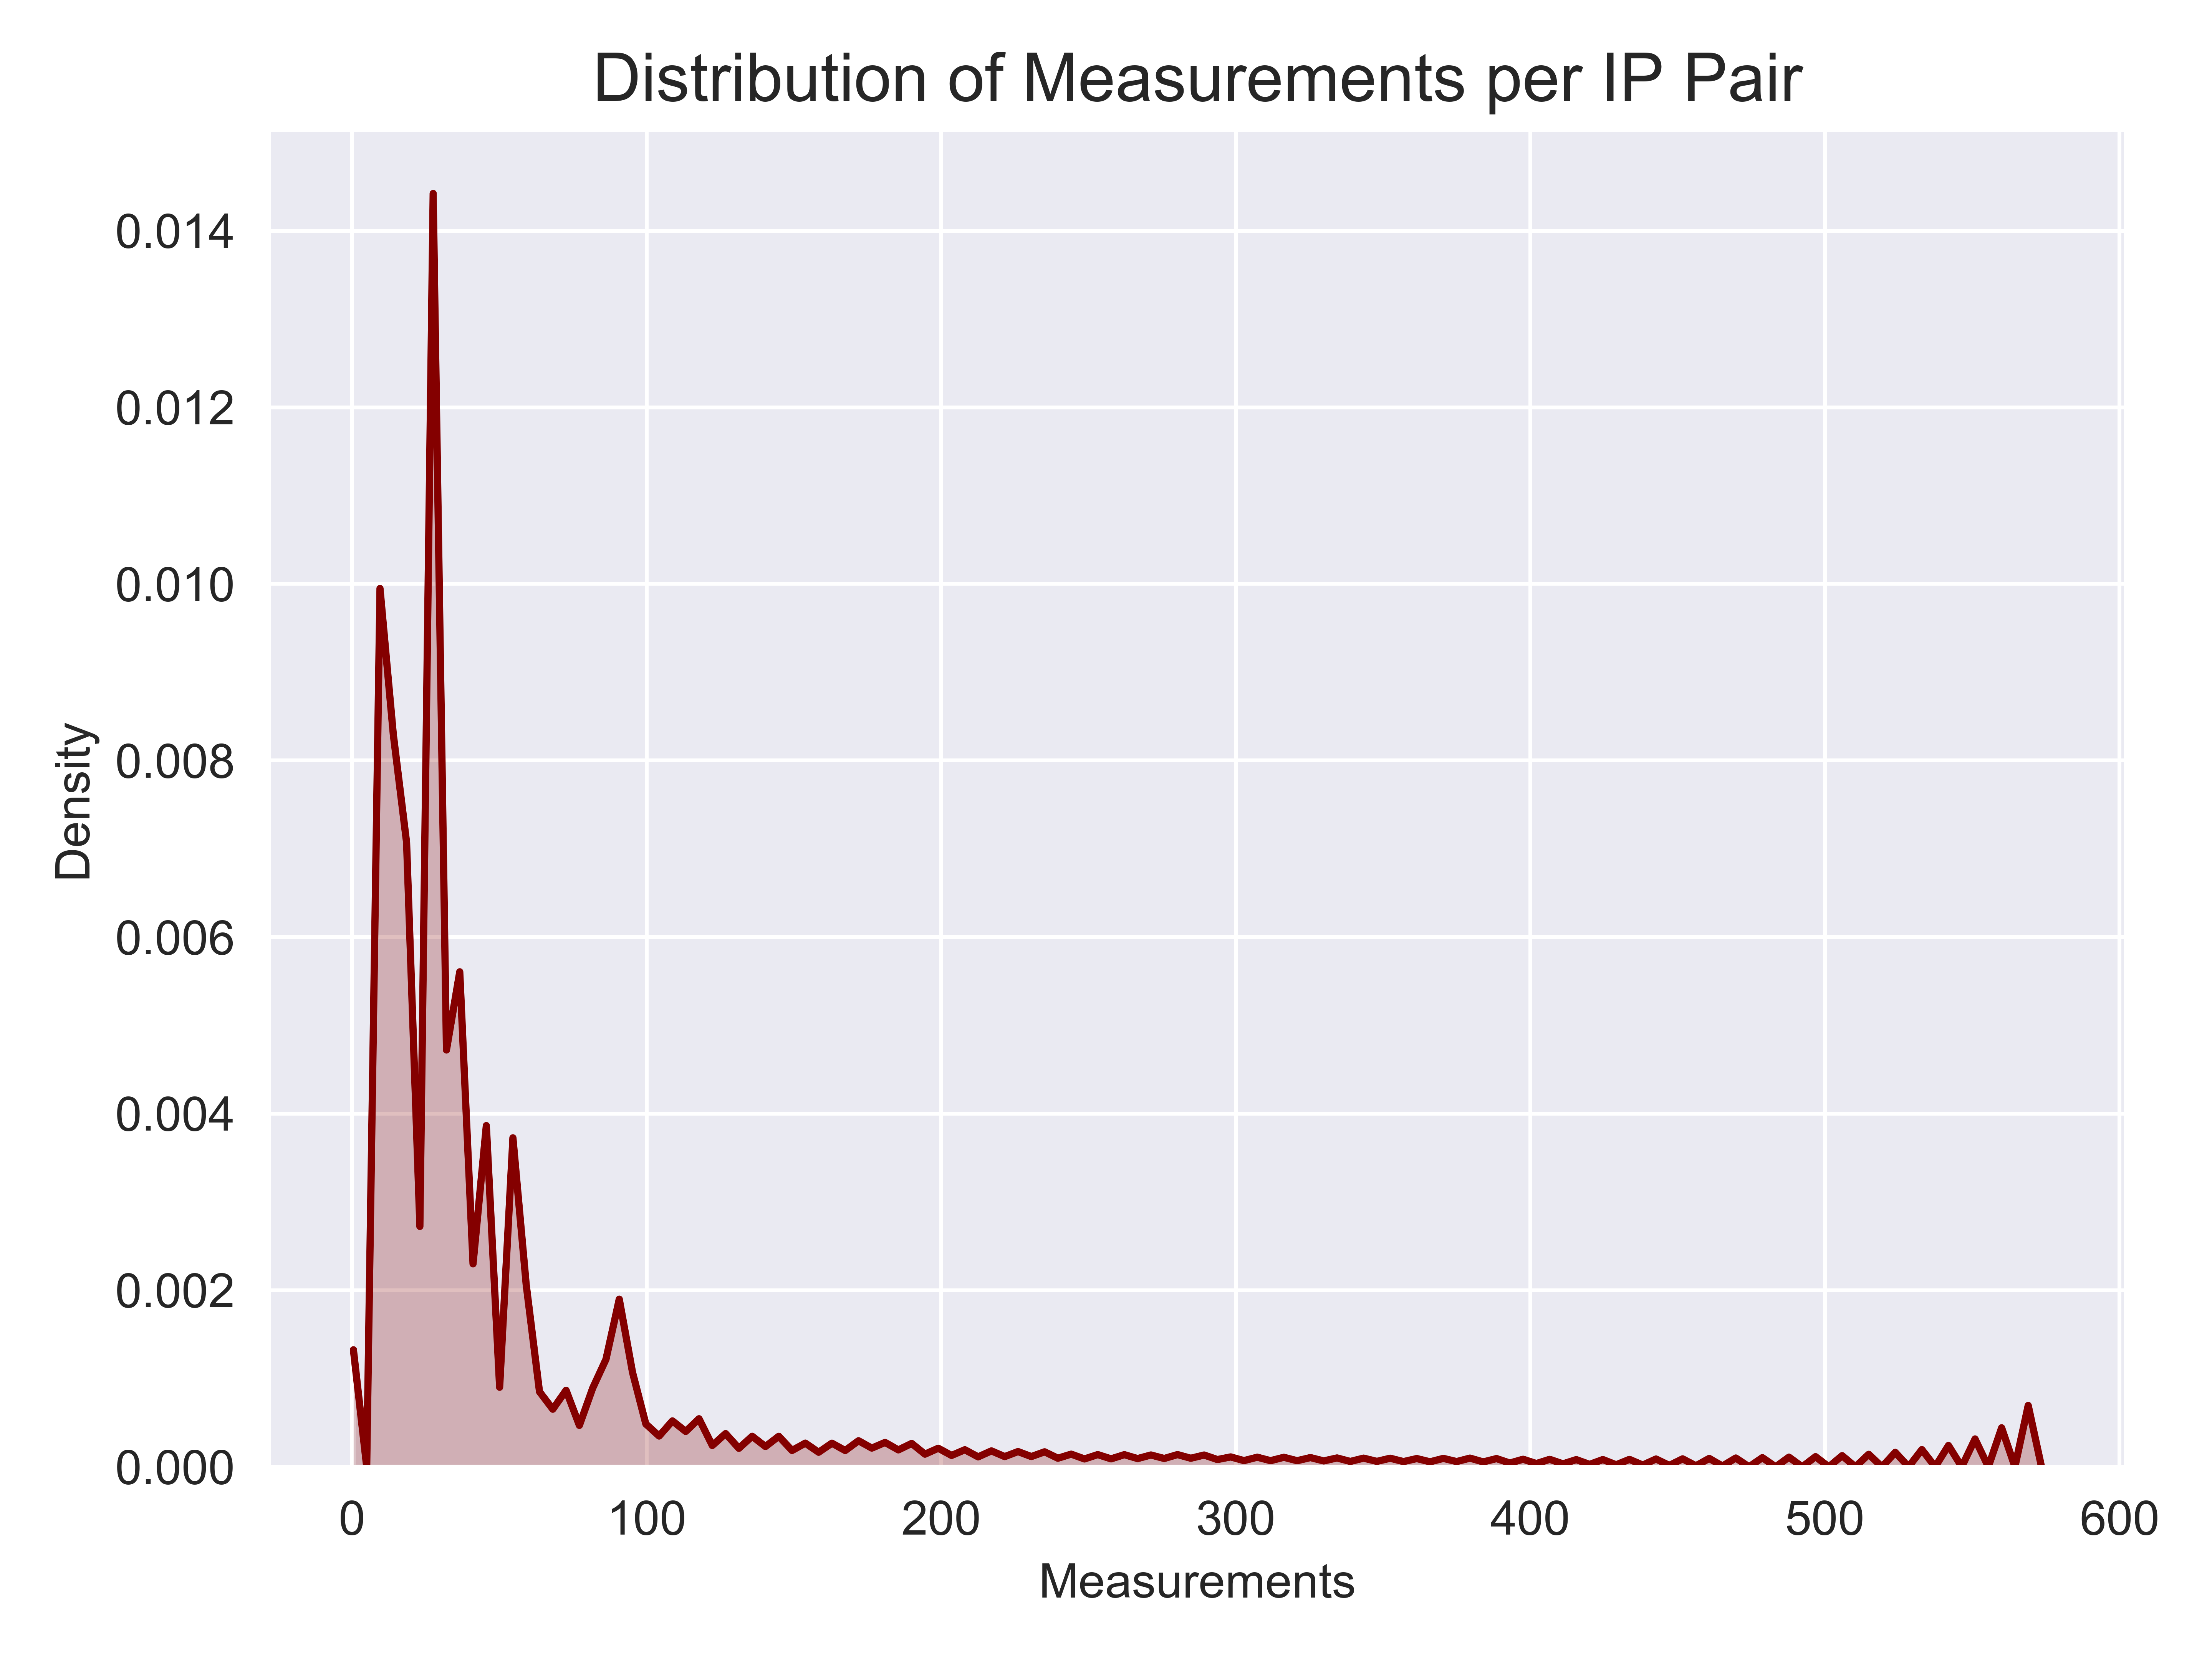
\includegraphics[width=0.65\textwidth]{caida/measurements_distribution.png}
    \caption{Distribution of measurements count for each address pair}
    \label{fig:caida_measurements_distribution}
\end{figure}
% \end{wrapfigure}

% \begin{wrapfigure}{L}{0.65\textwidth}
\begin{figure}[htb]
    \centering
    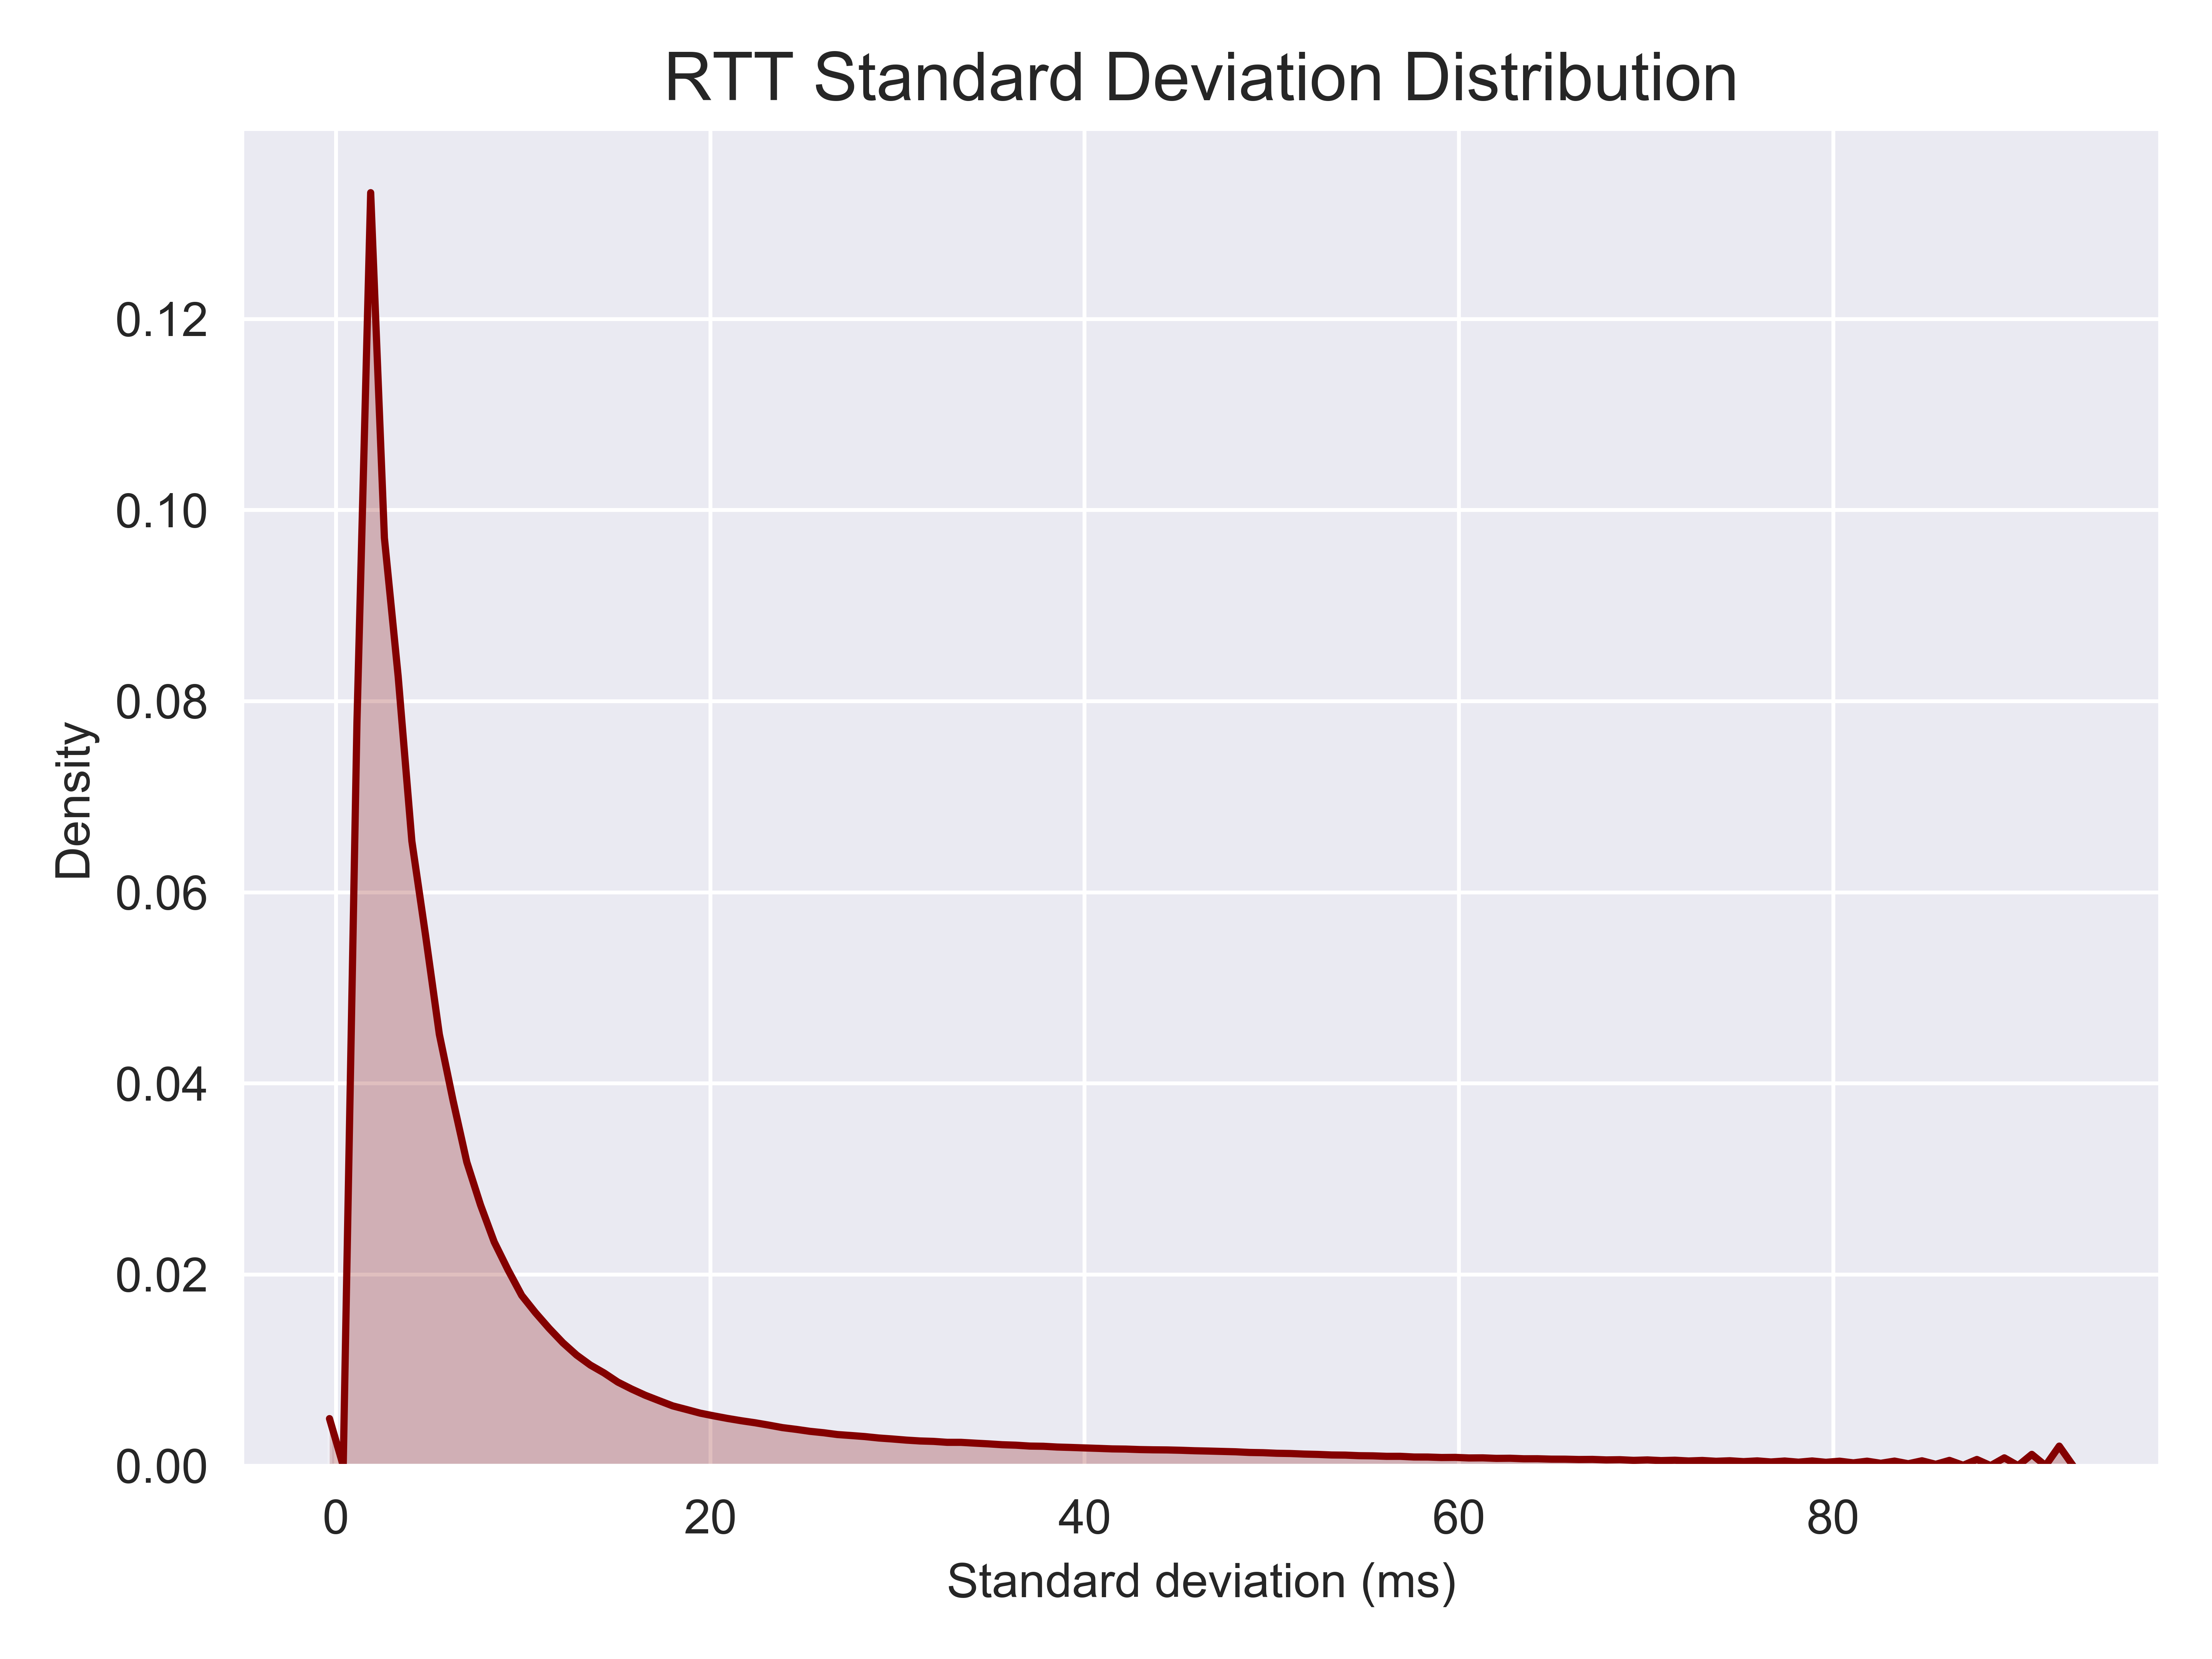
\includegraphics[width=0.65\textwidth]{caida/rtt_stdev_distribution.png}
    \caption{Distribution of address pair standard deviations}
    \label{fig:caida_stdev_distribution}
% \end{wrapfigure}
\end{figure}

The first measure of data quality used is standard deviation. \Cref{fig:caida_stdev_distribution} shows the distribution of standard deviations across all measured \ip address pairs (for charting purposes, pairs with only one measurement were interpreted as 0 standard deviation). The chart shows an incredibly smooth curve where the overwhelming majority of pairs have standard deviations well below 20 ms.

Since standard deviations are all relative, we next calculated a \cv for each \ip address pair as a measurement of data quality. \Cref{fig:caida_cv_distribution} shows the distribution of \cvs for all \ip address pairs, with the majority of \cvs below 0.1 -- in other words, excellent-quality data with low spread for each pair.

\begin{figure}[htb]
    \centering
    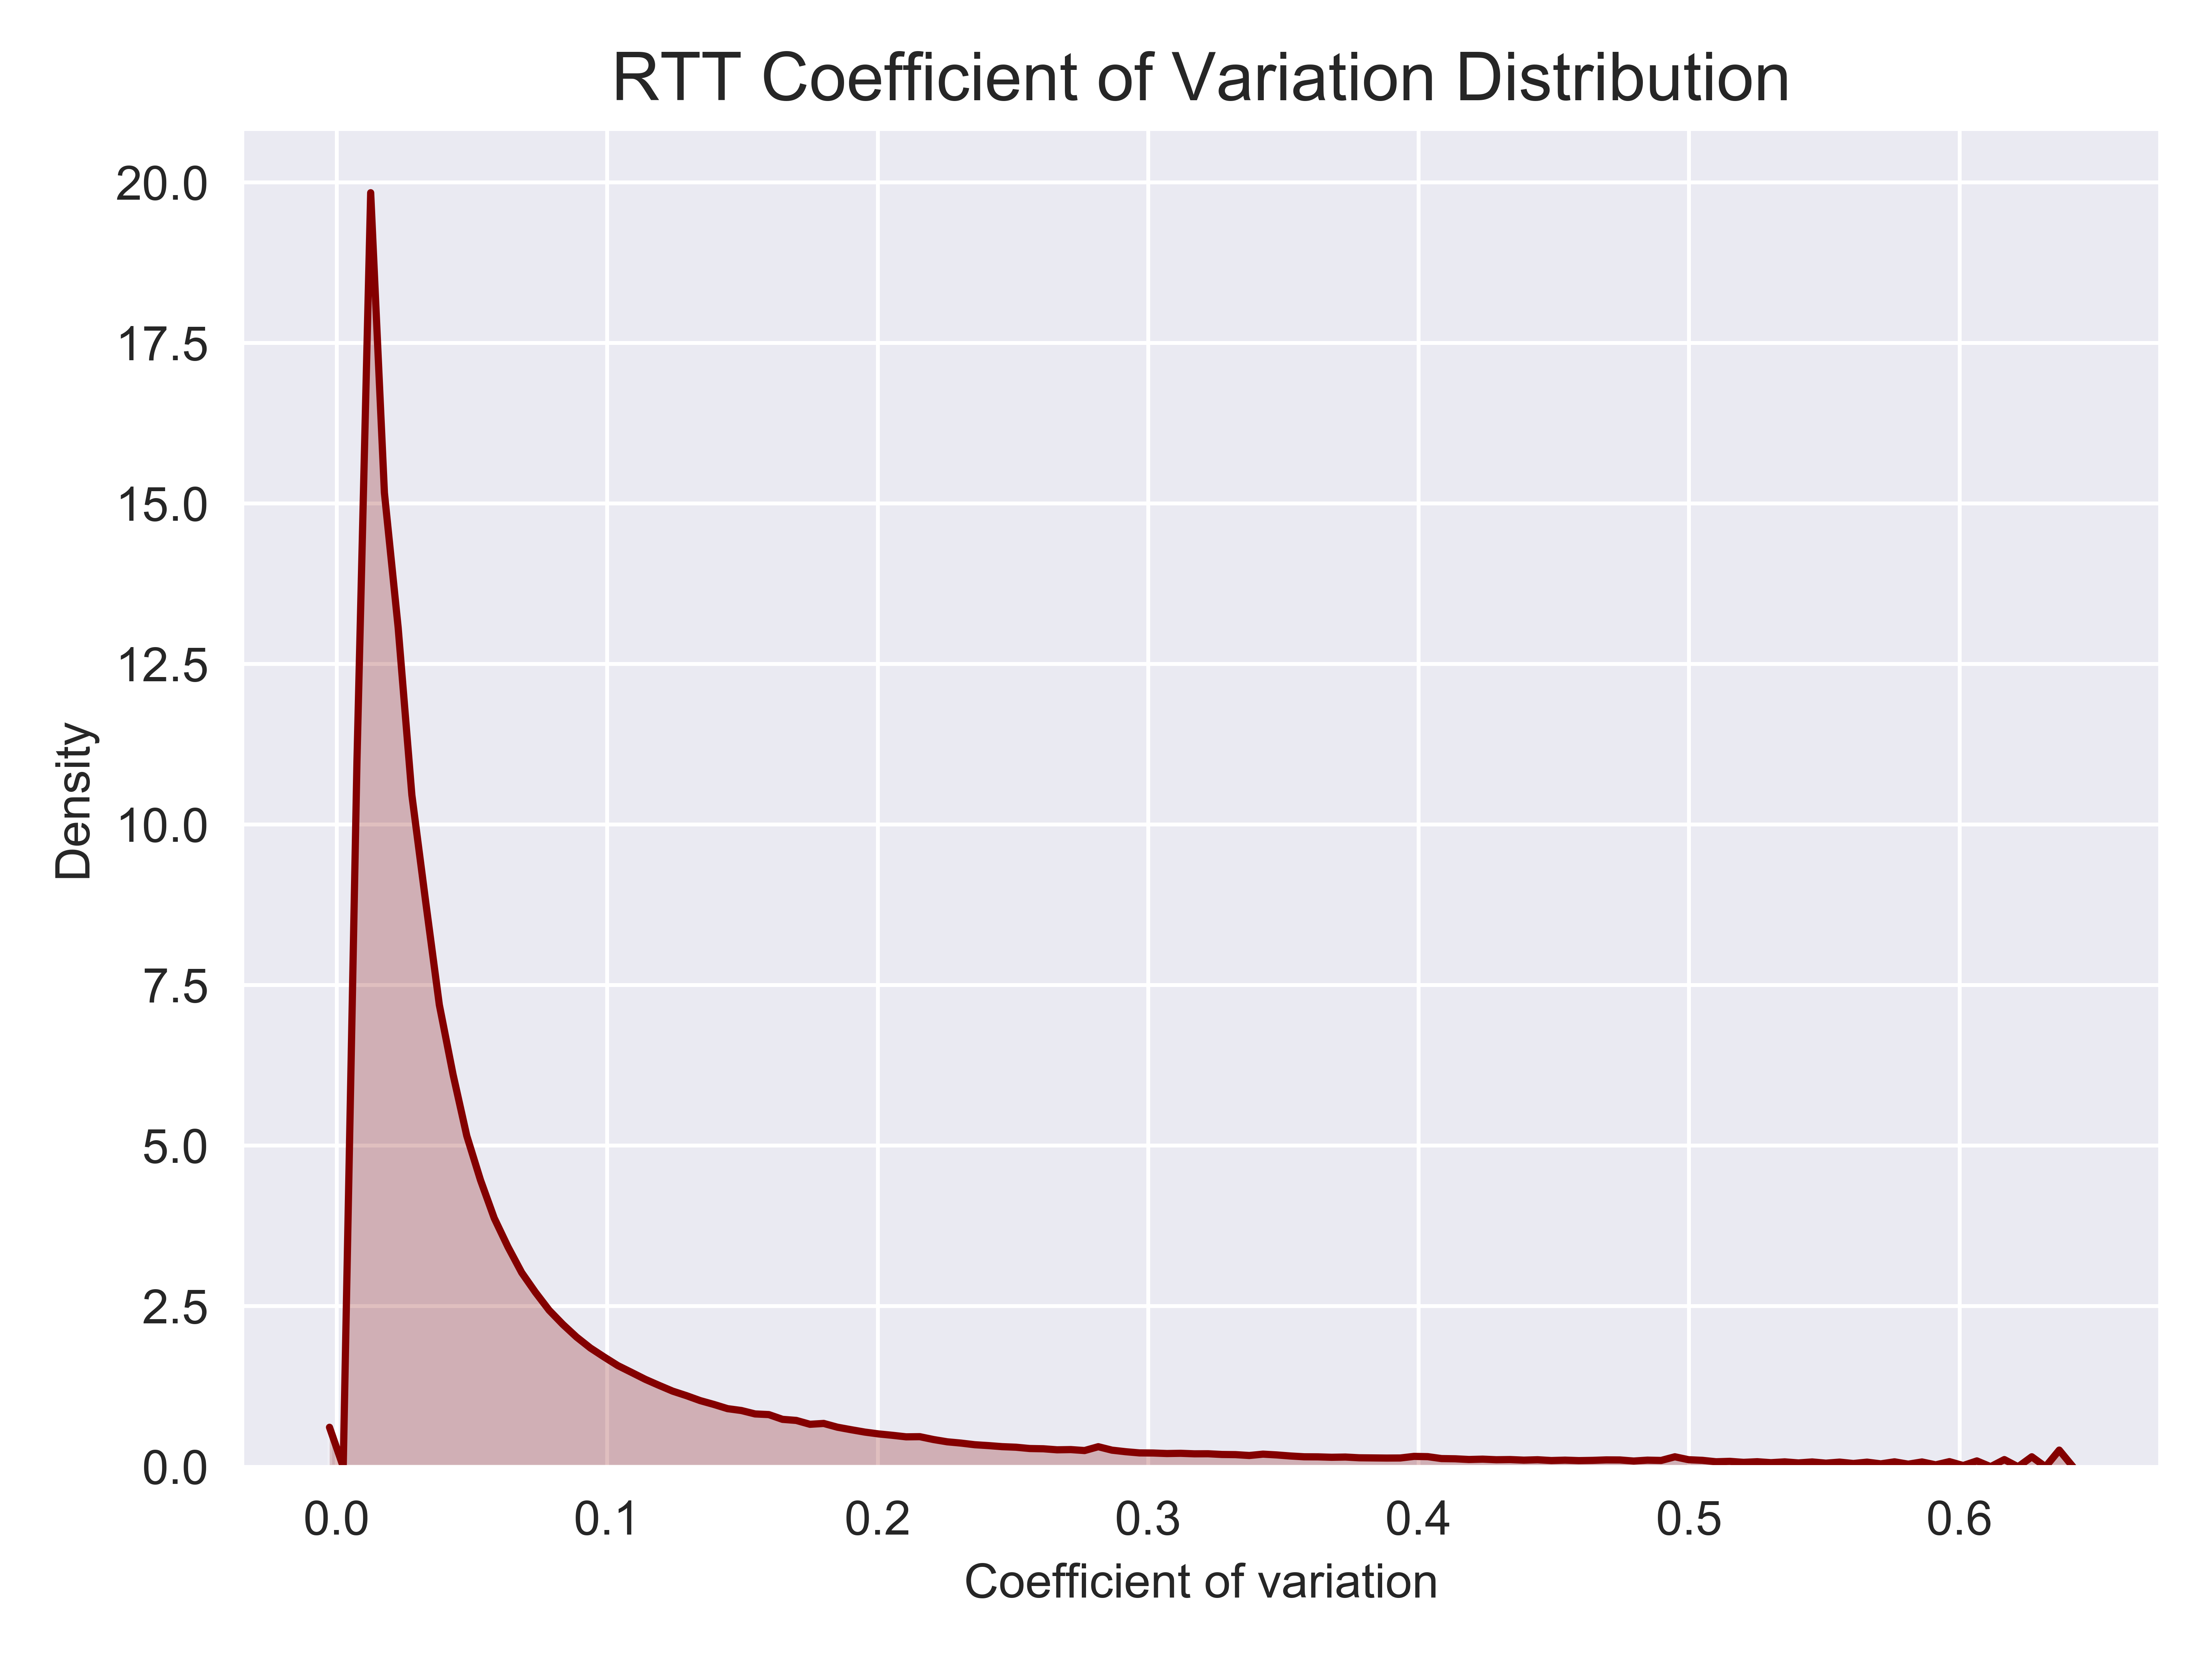
\includegraphics[width=0.65\textwidth]{caida/rtt_cv_distribution.png}
    \caption{Distribution of address pair coefficients of variation}
    \label{fig:caida_cv_distribution}
\end{figure}

\subsection{Primitive Connectivity Analyses}

Each data point comprises an \ip address pair, but each destination \ip address -- that is, each \ip address that a \caida or \ripe Atlas node ran a measurement against -- appears many times, at least once for every node that ran a measurement against it. Averaging these will not work (it makes little sense to average together measurements from a server in Boston with a server in Moscow against a server in New York, since the Moscow measurement node will naturally report a much higher \rtt), so normalization is needed. The first method used was simple normalization by distance, which returns values in ms/km. This may be unconventional, but milliseconds and kilometers are natural units for \rtts and distance, respectively.

\begin{figure}[htb]
    \centering
    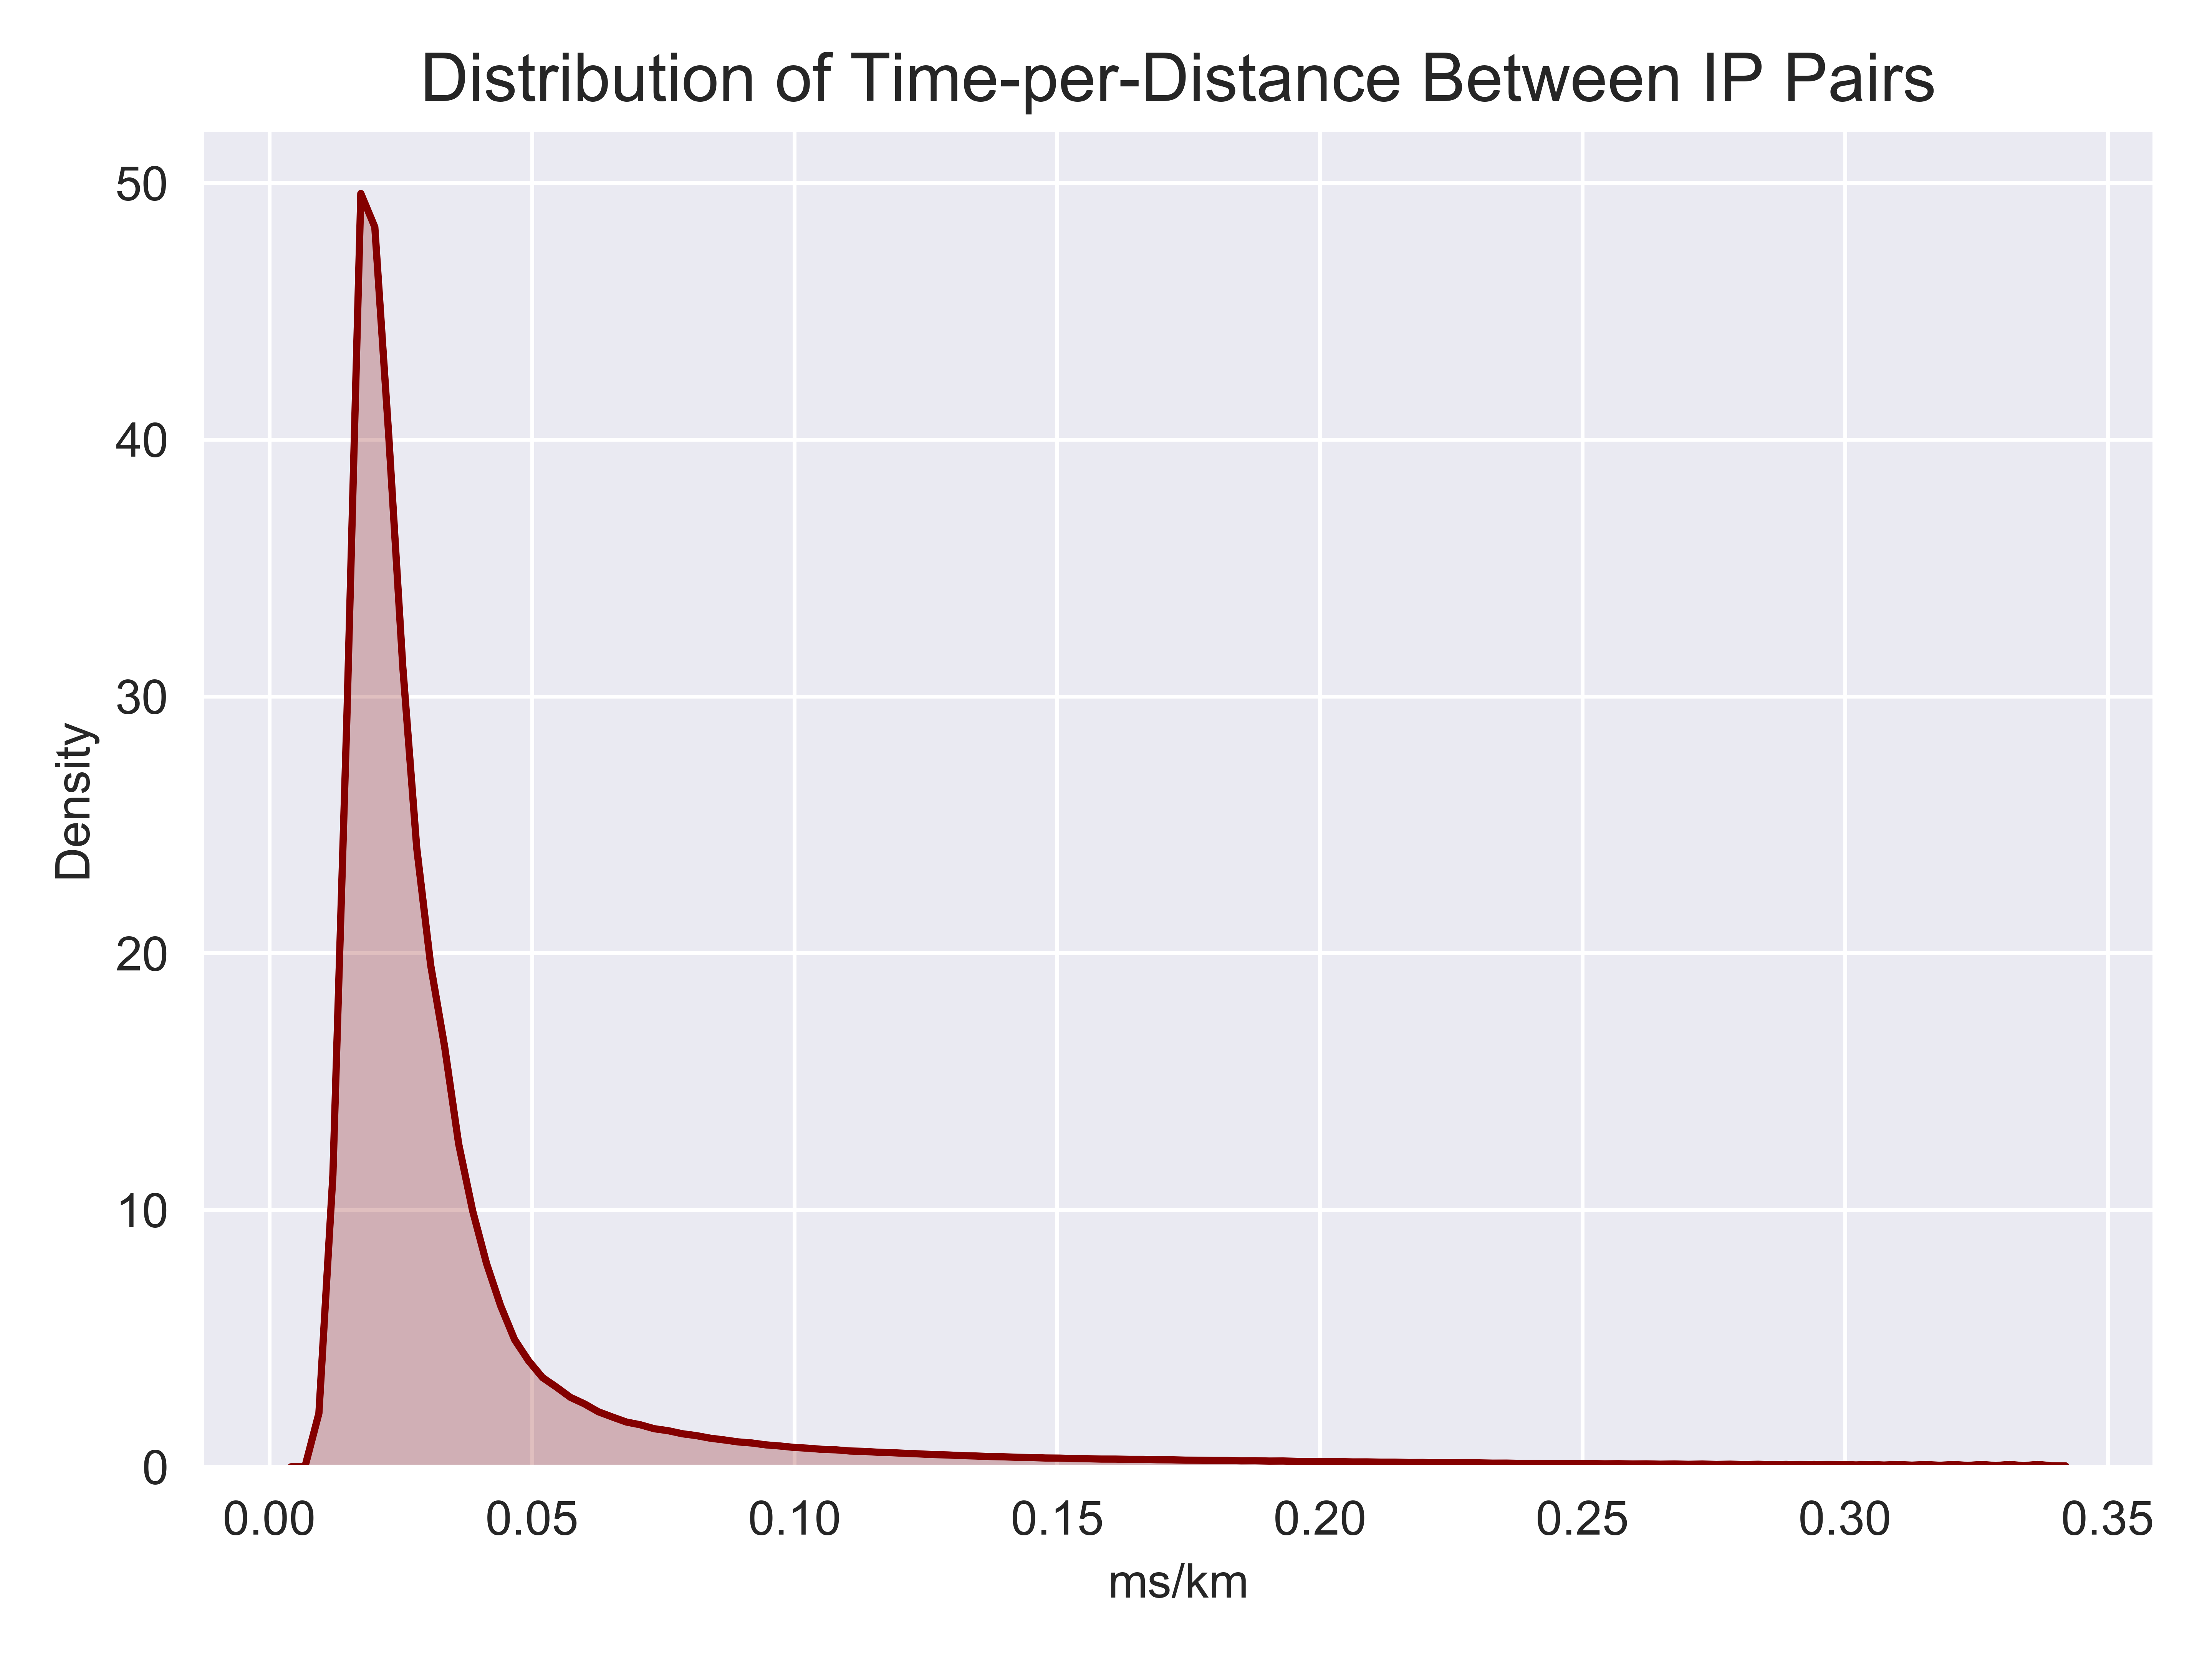
\includegraphics[width=0.75\textwidth]{caida/ms_per_km_distribution.png}
    \caption{ms/km connectivities distribution}
    \label{fig:caida_ms_per_km_distribution}
\end{figure}

The ms/km distribution shown in \cref{fig:caida_ms_per_km_distribution} is uninformative on its own, but it does demonstrate an important feature. Normalization succeeds in removing the bimodality of the \rtt distribution shown in \cref{fig:caida_rtt_distribution} without removing \textit{all} the spread of the data. This both further affirms the earlier hypothesis about the cause of the bimodality, and gives cause to believe that geographic charting may yield interesting results.

Unfortunately this metric is challenging to chart with any color scale. The majority of values are between 0.0 and 0.05 ms/km but values an order of magnitude higher must also be charted, and a log scale fails to capture important but relatively small variances between areas. To solve this, we devised a new metric based on efficiency relative to the speed of light.

The speed of light is 299.79246 km/ms, so the theoretical minimum \rtt between two points \textapprox300 km apart is \textapprox2 ms -- one ms one way, and another on the return trip. All telecommunications happen over electromagnetic mediums,\footnote{With the possible exception of \ipaoc, which has been successfully demonstrated \cite{rfc1149, BergenLinuxUserGroup2001a}} be it fibre optic cables or copper wires, so communications always have a transmission delay proportional to the speed of light. If the \rtt was higher than two milliseconds, there must logically be some loss in speed somewhere in the network, whether that means poor infrastructure or wiring that does not follow a straight line to its target -- either way, an inefficiency. The smaller the \rtt, the higher the efficiency, and vice versa. This has the desirable quality that extreme outliers are always between zero and one regardless of how high the \rtt is. The formula for speed-of-light-efficiency based on \rtts is shown in \cref{form:speed_of_light_efficiency}.

\begin{formula}[htb]
    \begin{equation}
        E = \frac{2d}{t \times 299.79246}
    \end{equation}
    \caption[Speed-of-light efficiency]{Speed-of-light efficiency; $E$ is efficiency as a scalar from 0-1, $d$ is distance in kilometers, and $t$ is the \rtt in milliseconds.}
    \label{form:speed_of_light_efficiency}
\end{formula}

Speed-of-light efficiency can also be thought of as a scalar multiplied by $c$, the speed of light -- it's the equivalent "speed" of a ping. With this improved normalization scheme to work with, the subtle differences and patterns like those in \cref{fig:speed_of_light_efficiency_distribution} can be seen in the data when mapped. Also important is that this normalization method provides another means of filtering data -- anything above 1.0 efficiency can be removed since it violates the laws of physics by exceeding the speed of light.

\begin{figure}[ht]
    \centering
    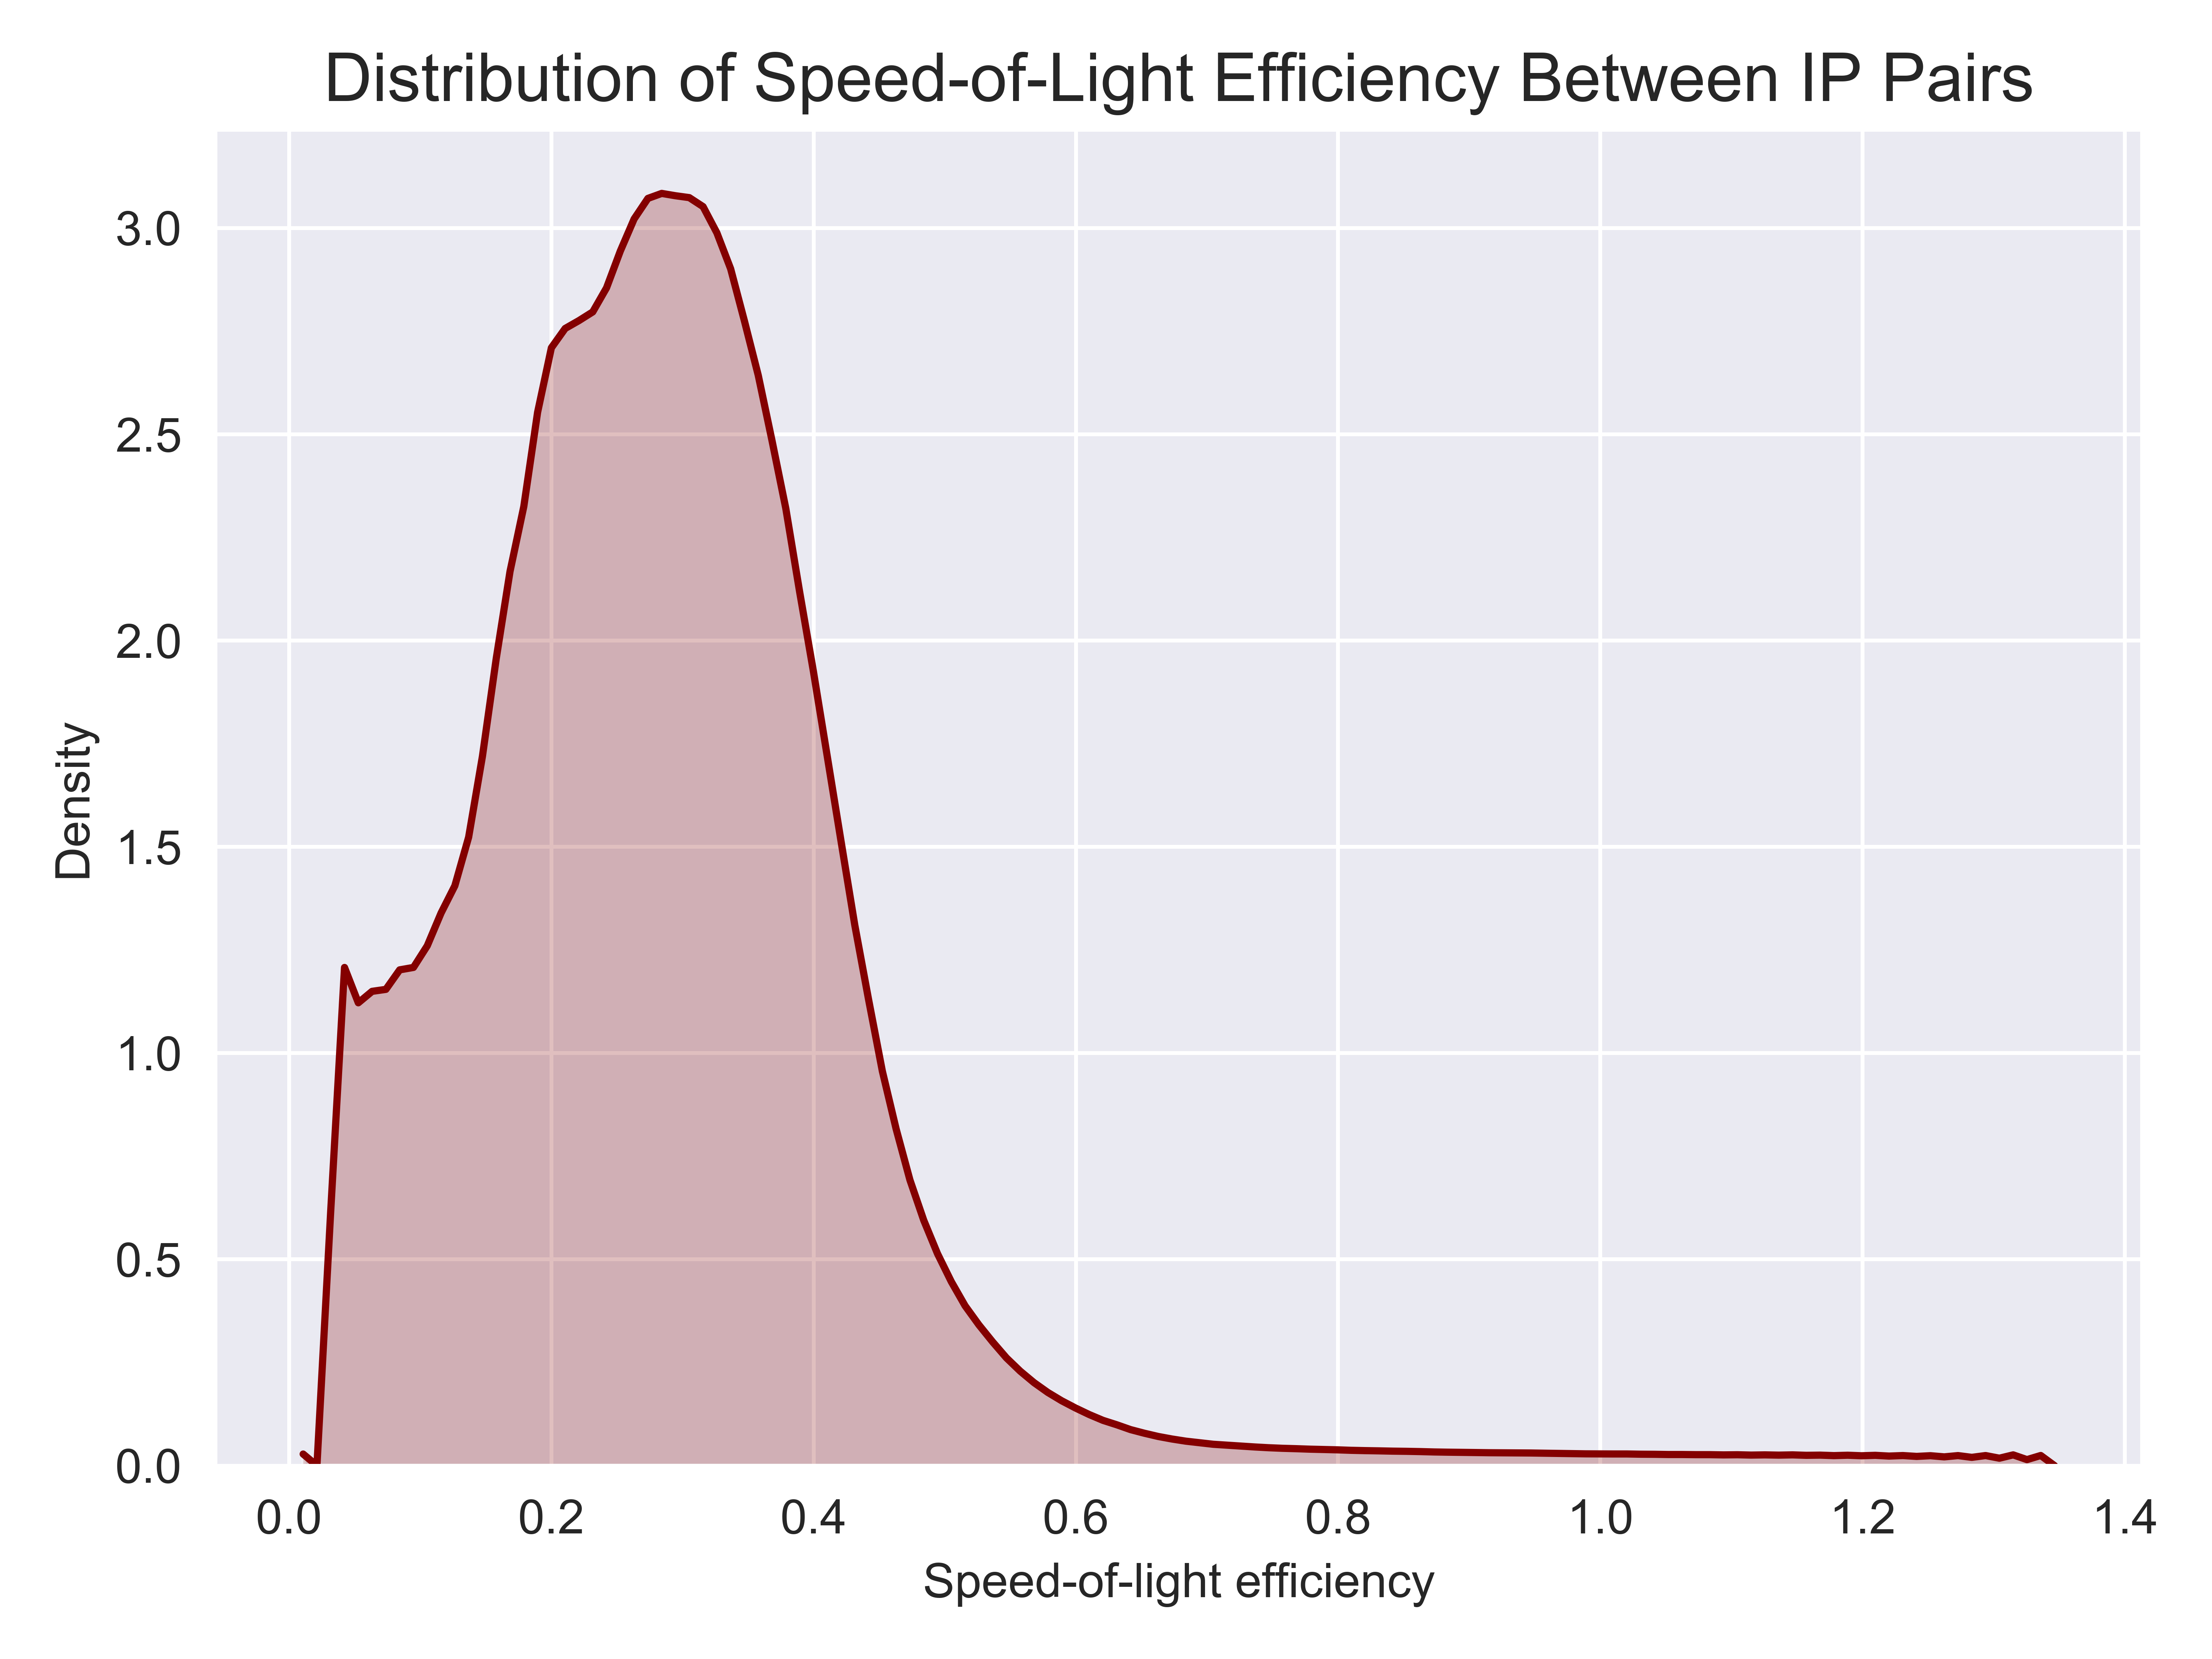
\includegraphics[width=0.65\textwidth]{caida/frac_c_efficiency_distribution.png}
    \caption{Speed-of-light efficiencies distribution}
    \label{fig:speed_of_light_efficiency_distribution}
\end{figure}

\subsection{Mapping}

The simplest way of mapping a set of points on a coordinate plane with values attached to each of them is a simple scatterplot, but with massive amounts of unevenly distributed data it becomes tough to visualize and draw conclusions. For example, in \cref{fig:caida_scatterplot} we see a point for \textit{every single pinged device} in the \caida and \ripe Atlas data set that was collected and analyzed -- at least, those in the \us.

\begin{figure}[htb]
    \centering
    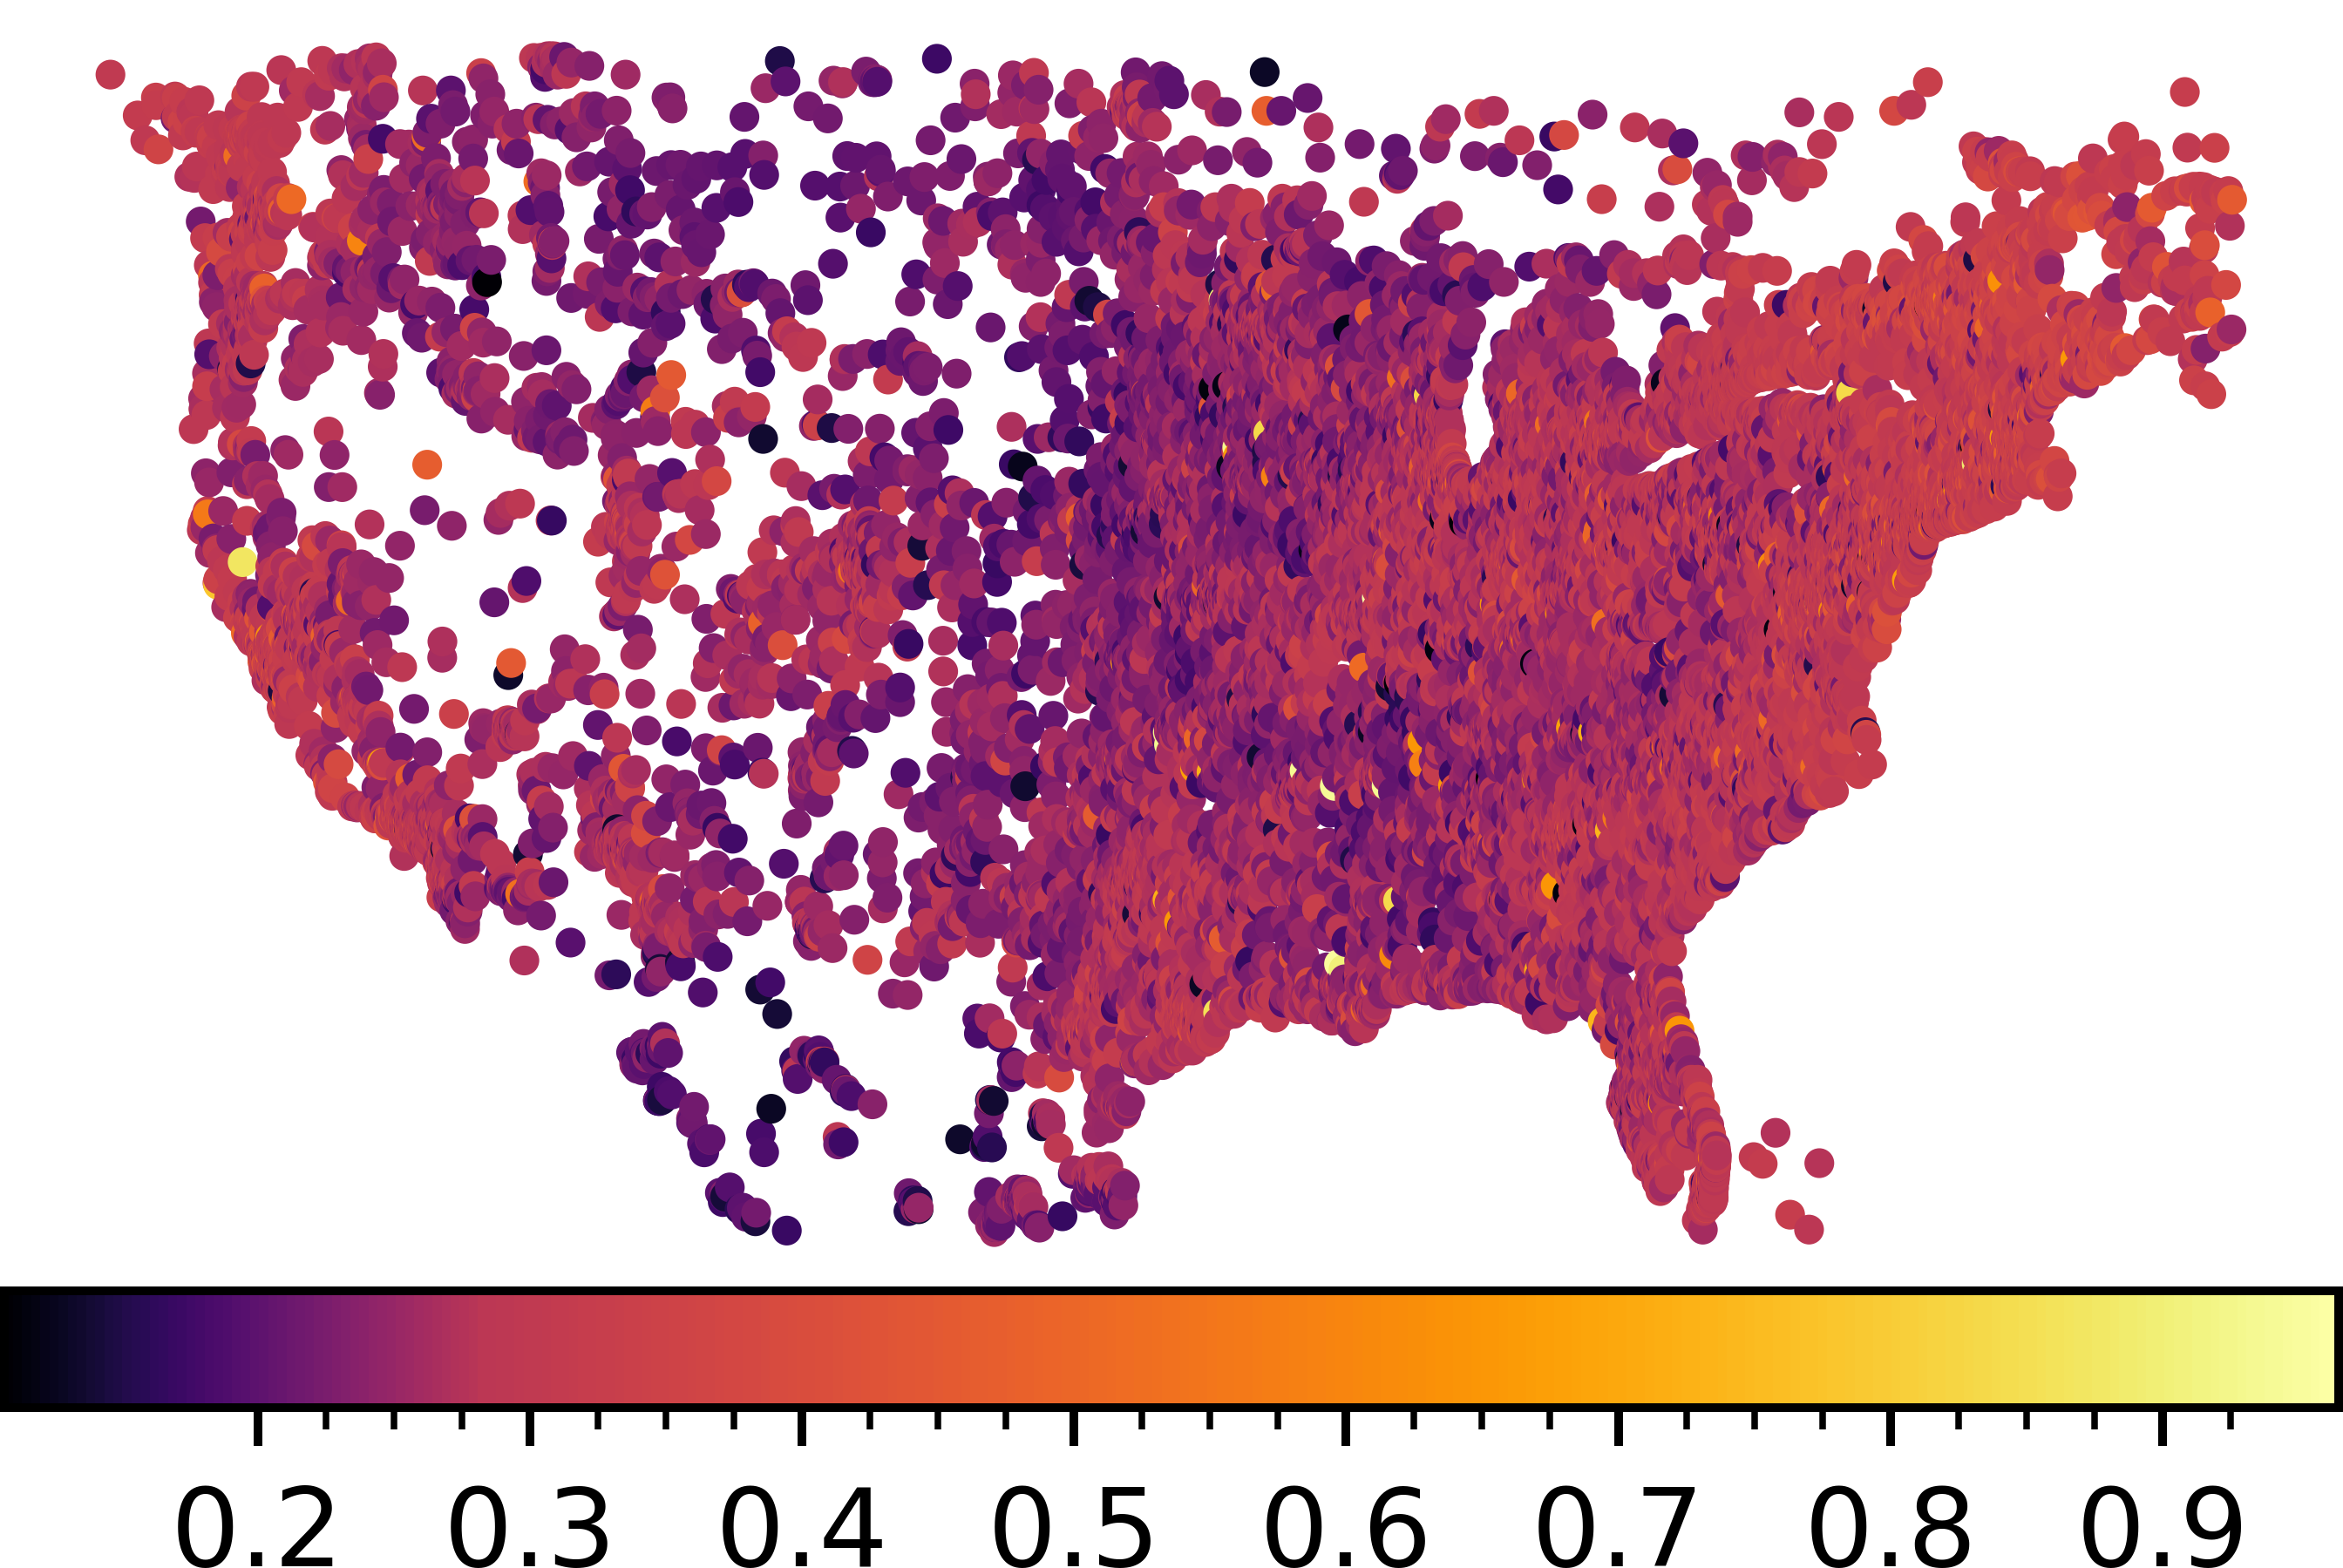
\includegraphics[width=0.65\textwidth]{caida/scatterplot.png}
    \caption{Traceroute scatterplot, colored by speed-of light-efficiency}
    \label{fig:caida_scatterplot}
\end{figure}

Some simple relationships can be inferred with moderate difficulty, like better internet connections near the coast or possibly major cities, but otherwise this map is only good at confirming that geolocation of IP addresses works. Many areas simply do not have measurements either, and those that appear covered look that way because the dots for each measurement were inflated for visual effect. If they were more accurately represented to-scale as single pixels, the map would be sparse.

To solve this problem the map needs some interpolation to fill in the gaps and make the data easier to understand. Ideally someone looking at the map should be able to point to a spot on the map and get an estimate for connectivity at that location, even if there was not a measurement at precisely that location. However, even after z-score filtering, aggregation by source-destination pairs, and more filtering, there were still millions of data points within the \us alone. To that end we tried some unusual techniques for further aggregating the data together, in ways that were more manageable for visualization tools. It was also decided that we should not lose resolution as the density of points increased. For example, drawing a grid of static boxes on top of the map and grouping using those would not do because there may be a city with thousands of points in one, and a rural area with only a few points in another, but they'd both take up the same area on the map.

\subsubsection{Quadtree grouping} One of the first techniques tried for grouping data together was a technique we dubbed "quadtree grouping". The technique is adapted from methods used to optimize collision detection in 2D games where the screen is cut into four boxes based on the number of entities in each quadrant, then each box is cut into four more with the same metric, and so on until some threshold with an optimal number of entities per box is reached. This process was performed on the data set here and adjusted for different parameters like maximum tree depth, maximum nodes per box, etc.

\begin{figure}[htb]
    \centering
    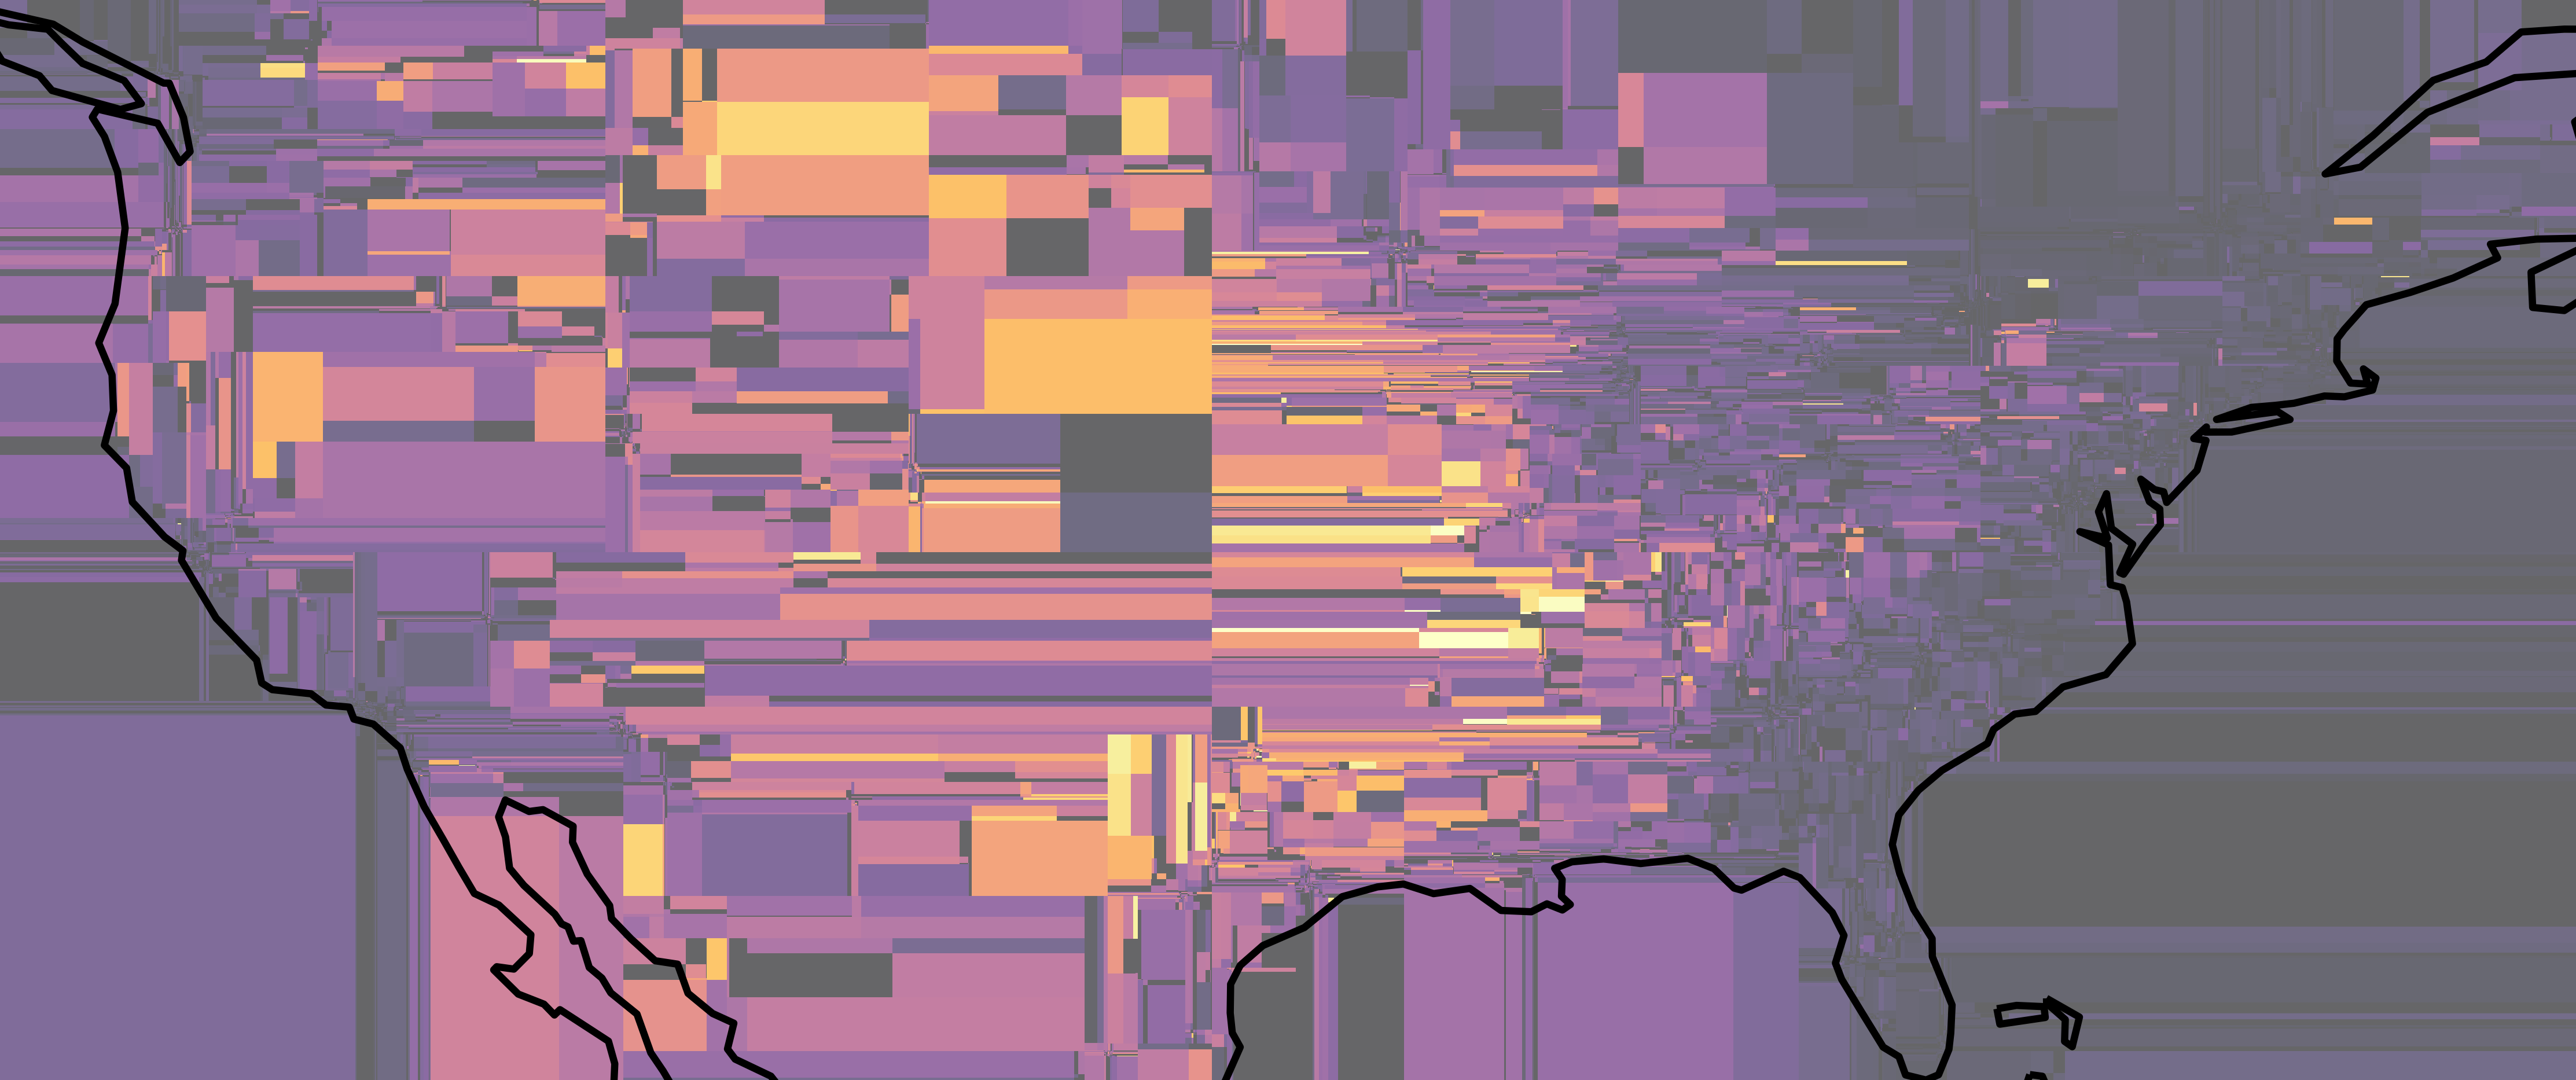
\includegraphics{caida/ms_per_km_quadplot.png}
    \caption{Traceroute ms/km quadplot, generated by quadtree grouping}
    \label{fig:quadtree_grouping}
\end{figure}

\Cref{fig:quadtree_grouping} shows a plot generated using this technique, with brighter areas corresponding to the higher \rtt-per-km metric, indicating worse connectivity. Smaller boxes tend to denote areas of higher population density, as they were areas the algorithm needed to subdivide the most. This technique appears to show a pattern in connectivity, with the East coast having overall better connectivity, but it's also visually difficult to read and difficult to interpret the data from -- it's displeasing to the eye.. The only way of assigning a single point to each quad is based on its center,\footnote{Technically it's possible to use some form of clustering within each quad to find an area with the highest density to pin the point on, but at that point you may as well just use clustering on the whole map.} but this results in points at odd positions, even out in the ocean.

\subsubsection{Nearest-neighbor interpolation}

At this point it was discovered that, due to the fairly low resolution of \ip address geolocation, many measurements from different \ip address pairs share the same coordinates. This made even further grouping by location possible, down to only \textapprox55,000 data points. This is much more manageable to visualize, so the next interpolation method tried was simple nearest-neighbor interpolation (which prior to grouping would have been infeasible).

\begin{figure}[htb]
    \centering
    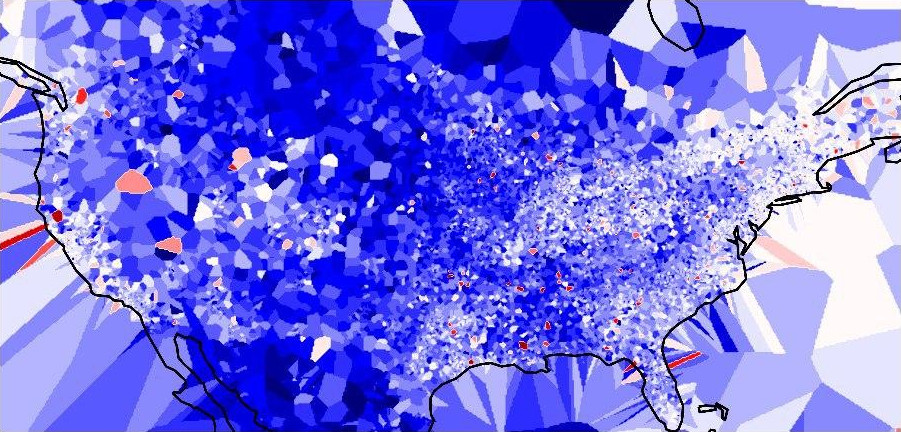
\includegraphics{caida/nearest_neighbor.jpg}
    \caption{Traceroute speed-of-light efficiency nearest-neighbor diagram}
    \label{fig:caida_nearest_neighbor}
\end{figure}

\Cref{fig:caida_nearest_neighbor} shows a nearest-neighbor plot, otherwise known as a Voronoi diagram \cite{Malhotra2017a}, of the \caida and \ripe Atlas data combined, generated with Python \textit{matplotlib} and \textit{scikit-learn} \cite{scipy, matplotlib}. The colormap is a divergent linear colormap, where blue is worse-than-average and red is better-than-average efficiency. This does an arguably better job of presenting the data than quadtree grouping, but it's visually noisy and suffers from expanded influence of points in sparse areas. For instance, consider the large splotch in Utah, which corresponds to areas arounhd Salt Lake City. While it's likely accurate that the city has far better internet connectivity than its desert surroundings, it is likely inaccurate to say that the areas within the few hundred mile radius shown on the map have the same level of connectivity.

\subsubsection{Linear interpolation}

Since nearest-neighbor interpolation proved insufficient, the next method tried was linear interpolation. Instead of assuming that all points nearer to a given data point than any other have the same value as the data point does, linear interpolation assigns values at each point between the different data points according to a simple linear scaling model. This has the effect of making the map look far less discrete.

\begin{figure}[htb]
    \centering
    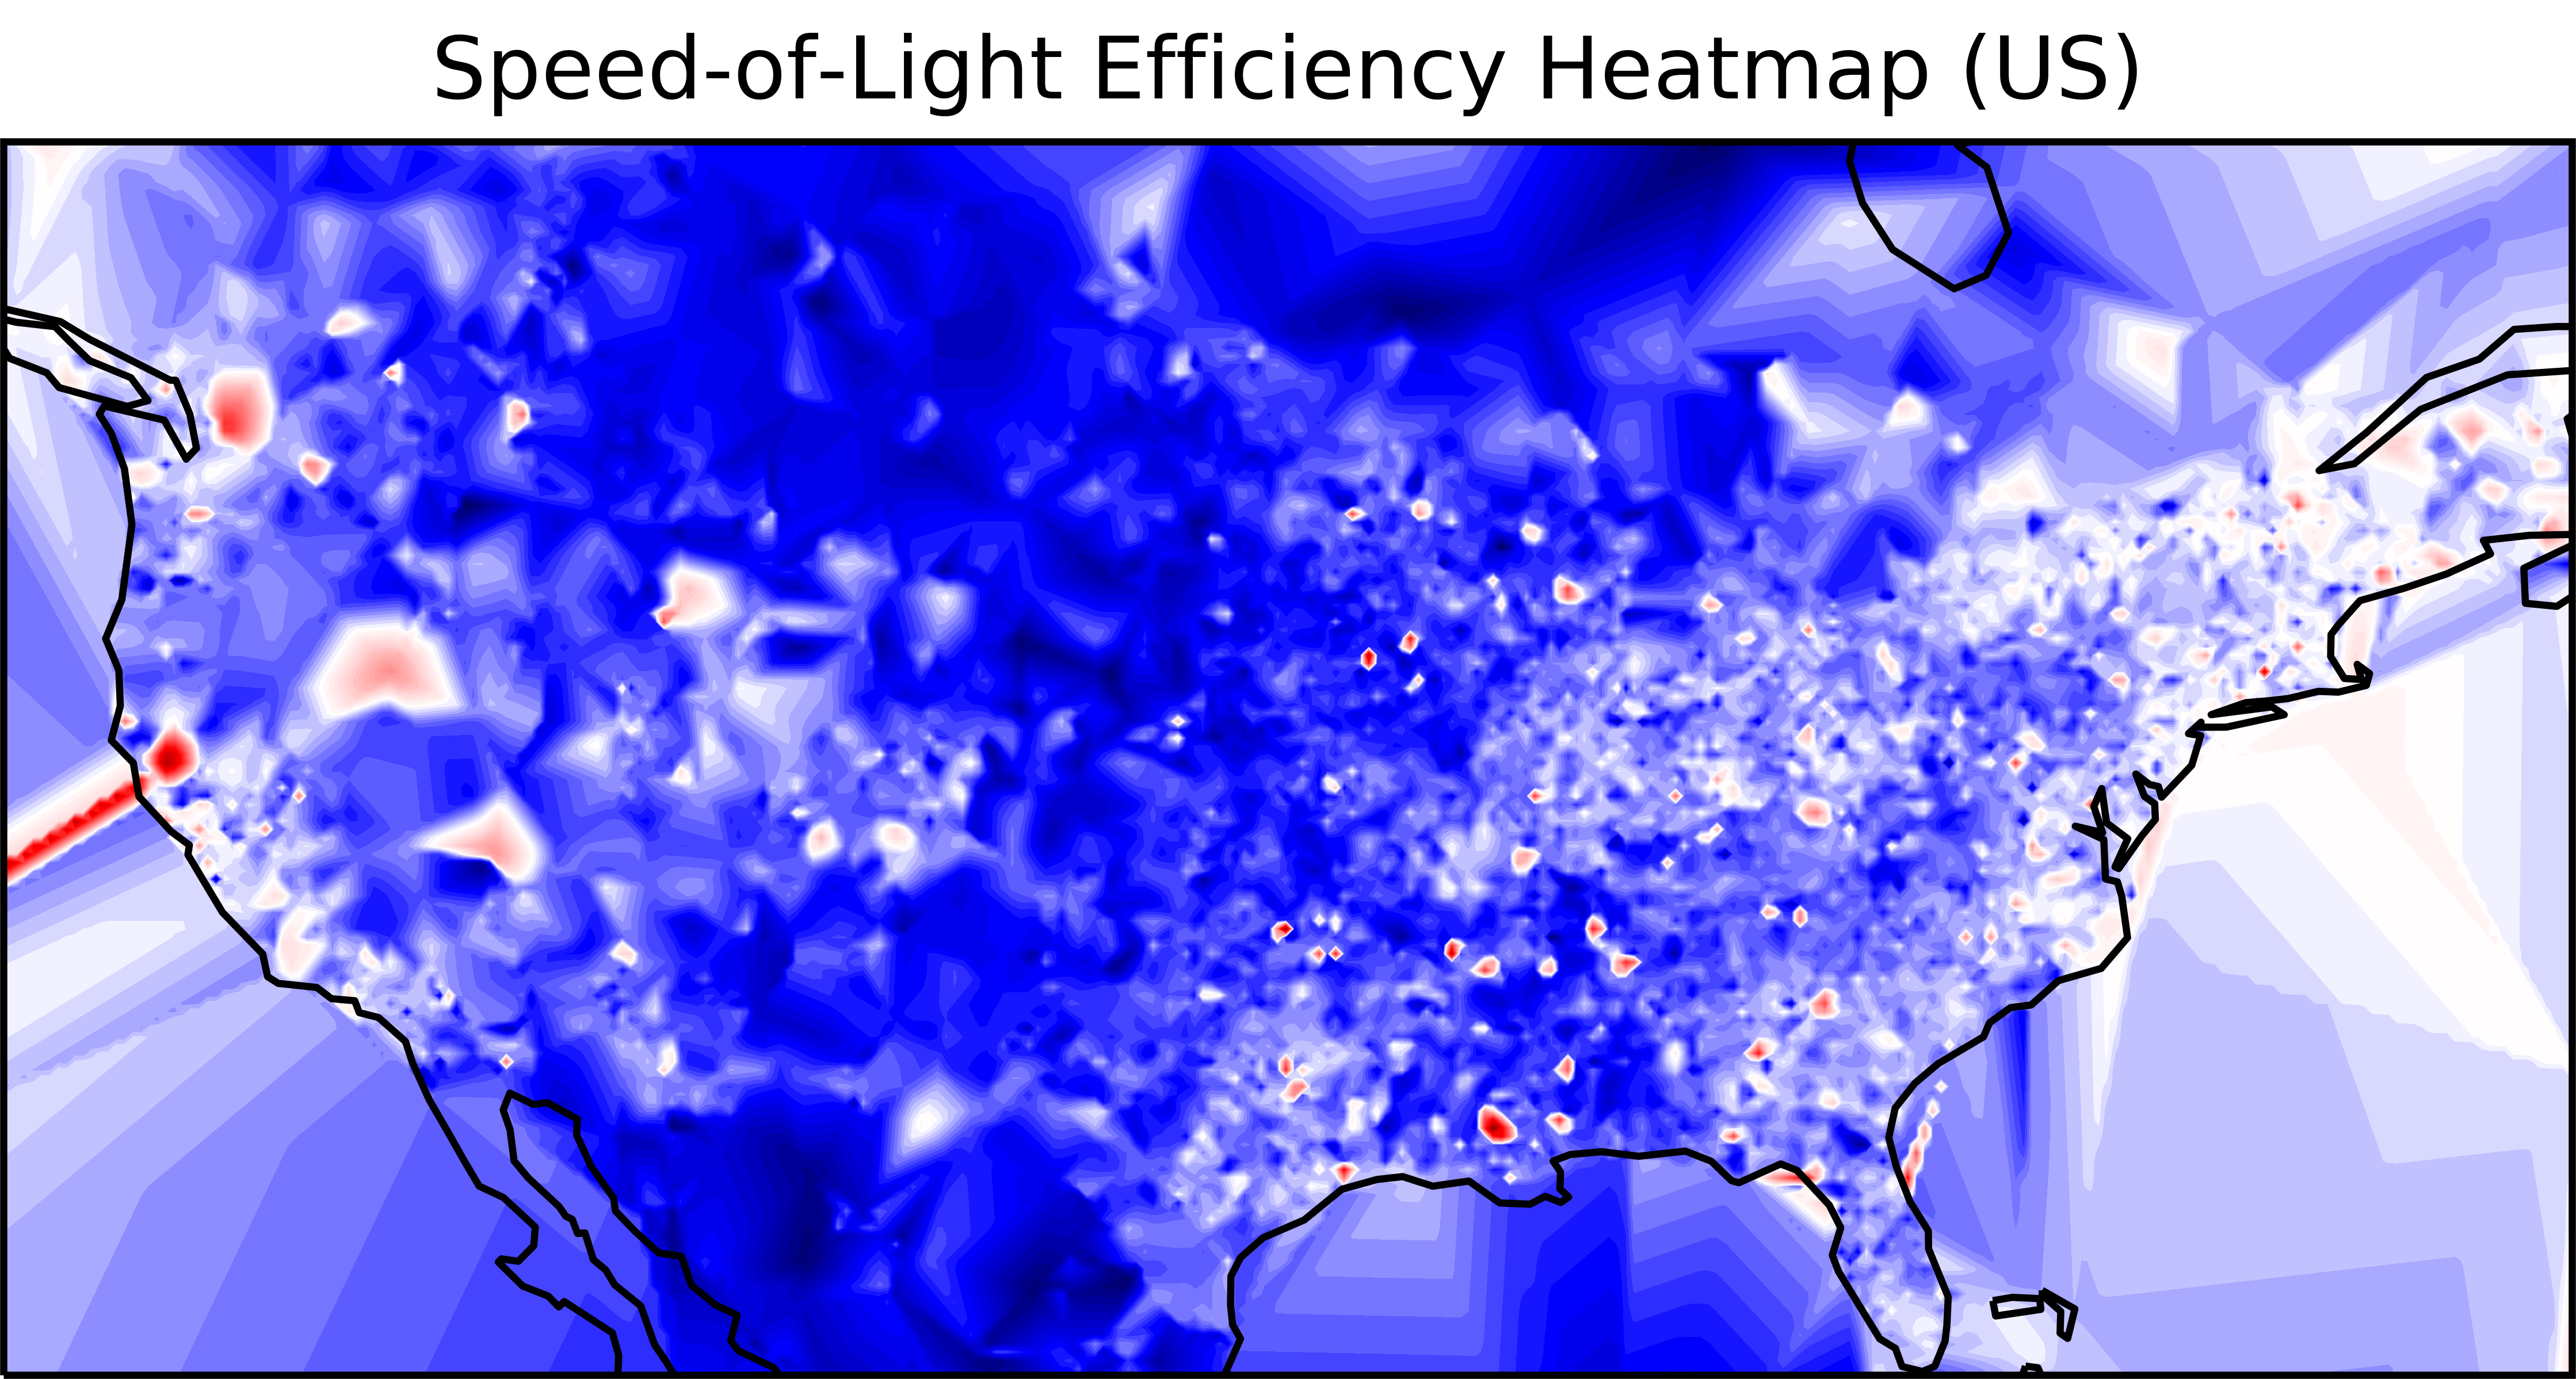
\includegraphics{caida/frac_c_efficiency_linear_divergent_heatmap.png}
    \caption{Linear-interpolated traceroute speed-of-light efficiency heatmap}
    \label{fig:caida_linear_interpolation}
\end{figure}

\Cref{fig:caida_linear_interpolation} uses the same divergent colormap as \cref{fig:caida_nearest_neighbor} but with linear interpolation instead, showing a far smoother map that preserves the same patterns. It does not look as discrete but it still has an angular affect to it, with sharp angles showing through where Voronoi cell bounds and intersections previously were.

\subsubsection{Inverse Distance Weighting}

\IDW is a method for interpolating point data, operating under the assumption that areas closer together are more likely to be similar. The influence of any given point on the interpolated data falls off with the inverse of the distance to that point, producing much smoother, much more easily understood (and likely more accurate) results.

\Cref{fig:caida_idw_heatmap} shows the data as interpolated with \idw and touched up to include state lines, major cities, and a key. This is what we consider to be the final heatmap generated from the \caida \& \ripe Atlas data. It roughly confirms our expectations that the more densely-populated coasts would have have better connectivity on average while adequately highlighting large-scale trends.

Interestingly, no matter how the data is visualized it always has a great deal of variance from one area to another -- that is, the map looks "splotchy". Loosely speaking, this is also what we would expect to see, since people tend to report a great deal of subjective difference in internet quality from one area to another.

\begin{figure}[htb]
    \centering
    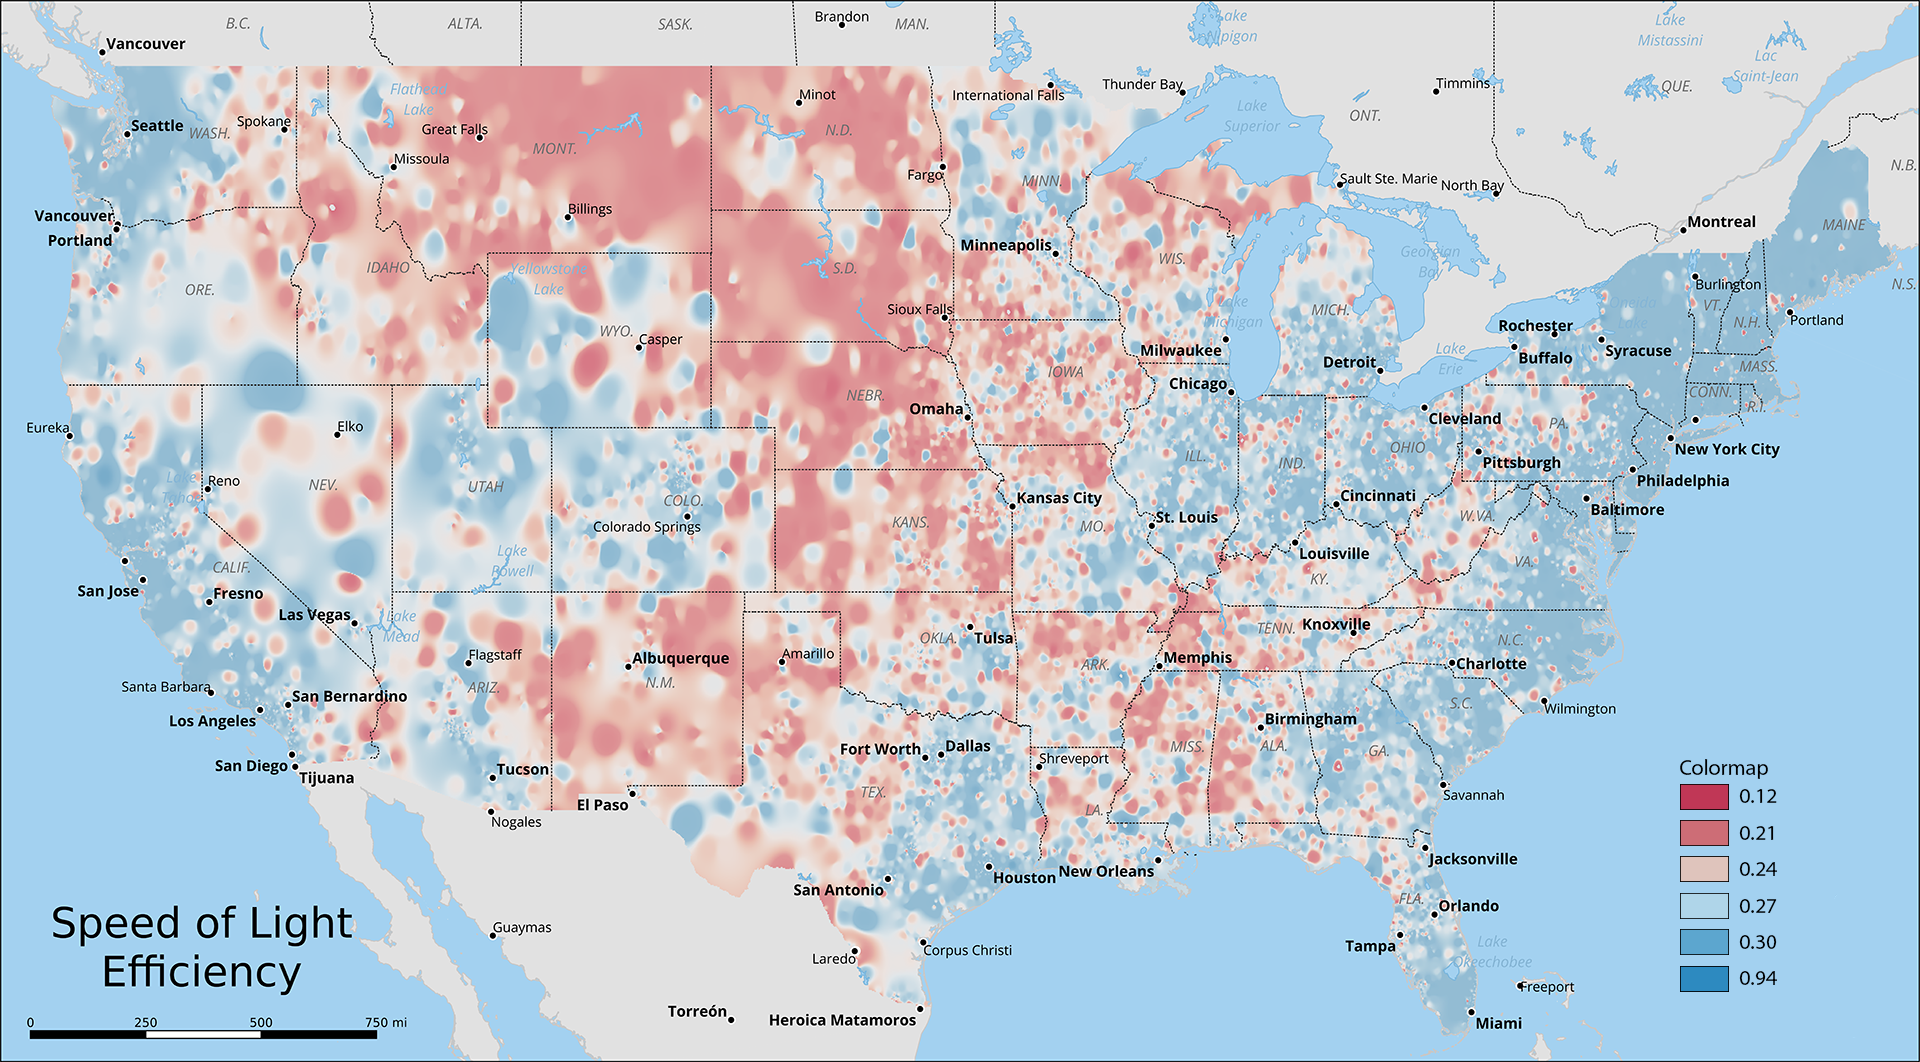
\includegraphics{caida/speed_of_light_idw.png}
    \caption{Inverse distance weighting traceroute speed-of-light efficiency heatmap}
    \label{fig:caida_idw_heatmap}
\end{figure}
